% kapitel4.tex
\externaldocument{02_grundlagen.tex}
\externaldocument{03_fragestellung}
\chapter{Implementierung}
\label{chapter:implementierung}
Der folgende Abschnitt stellt die in Abschnitt~\ref{section:steurungsmodell} beschriebenen Modelle und ihre Implementierung im entwickelten Softwareprototyp dar. Zunächst wird auf die optischen Eigenschaften des Softwareprototyps eingegangen. Im Anschluss erfolgt eine Beschreibung der beiden technischen Komponenten des Systems sowie ihre Implementierung. Hierzu zählen das \et \iV der Firma \acf{smi} und das verwendete mobile Robotersystem (Roomba 620) der Firma iRobot® Corporation.

\section{Gestaltung der Benutzeroberfläche}
\label{sect:gui}
In Bezug auf die Erstellung einer grafischen Benutzeroberfläche (engl. \acf{gui}) wurde die grundlegende Struktur des Vorgängersystems von Eidam übernommen und um Elemente der Robotersteuerung und der Kameraverbindung erweitert, \vgl~\cite{Eidam2015}. Nachfolgend werden zusammenfassend die bestehenden Komponenten beschrieben. Der Fokus liegt auf den zur Vorgängerarbeit erweiterten Komponenten, explizit auf den Steuerungskomponenten.

\subsection{Allgemeine Komponenten der Benutzeroberfläche}
\acl{abb}~\ref{fig:diskretModeKomp} zeigt die vier wesentlichen Komponenten, die im Rahmen des Softwareprotyps verwendet wurden. Hierzu zählen die Menüleiste (1. rote Markierung), die Steuerelemente (2. gelbe Markierung, hier diskrete Steuerelemente), eine Statusleiste (3. blaue Markierung) und die aktuelle Darstellung der Kamerasicht (4. grüne Markierung). %Der \acs{por} des Benutzers erscheint als rot markierter Punkt im Zentrum der Darstellung und bewegt sich in Abhängigkeit der Blickbewegung.

\begin{figure}[ht]
\begin{center}
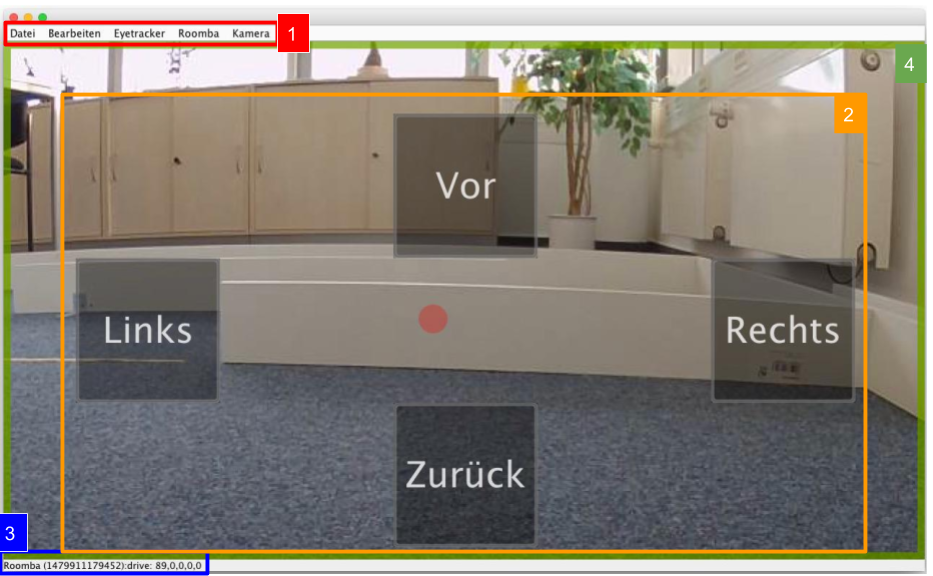
\includegraphics[width=0.7\textwidth]{bilder/implementierung/diskretMode1.png}
\end{center}
\caption{Darstellung der wesentlichen Komponenten des Softwareprototyps. (1)~Menüleiste mit den Punkten: Datei, Bearbeiten, Eyetracker, Roomba, Kamera. (2)~Steuerelemente (hier diskrete Steuerelemente). (3)~Statusleiste. (4)~Kamerapanel mit der Ansicht aus Sicht des mobilen Roboters. Der \acs{por} des Benutzers im Zentrum der Darstellung  erscheint als rot markierter Punkt.}
\label{fig:diskretModeKomp}
\end{figure}

Die Menüleiste (siehe \acs{abb}~\ref{fig:menu}) beinhaltet im Menüpunkt \enquote{Datei} neben der Möglichkeit, die Software zu starten und zu beenden, die Option, relevante Einstellungen in Bezug auf die Systemnutzung vorzunehmen. Der Menüpunkt \enquote{Eyetracker} ermöglicht,- neben dem Starten und Stoppen des Eyetrackings,- auch die vor jeder Nutzung notwendige Kalibrierung des Eyetrackers. Des Weiteren kann der \acs{por} an- \bzw ausgeschaltet werden. Auch die Möglichkeit, in einem Simulationsmodus den Eyetracker mit der Maus zu simulieren, ist gegeben. Ein Lidschluss kann dabei mit der rechten Maustaste simuliert werden \cite{Eidam2015}. Der Menüpunkt \enquote{Roomba} ermöglicht, die verbindungsrelevanten Einstellungen des mobilen Roboters (Roomba) anzupassen. Ferner wird die Möglichkeit des Resets und des Fahrens zur Ladestation gegeben. Der letzte Menüpunkt \enquote{Kamera} ermöglicht es, die kamerarelevanten Einstellungen vorzunehmen und anzupassen.
\begin{figure}[ht]
\begin{center}
   \begin{minipage}[t]{.4\linewidth} 
      \centering 
      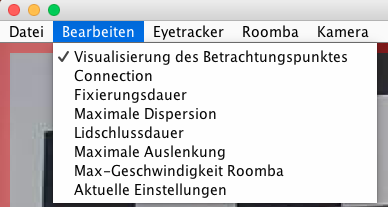
\includegraphics[width=1\textwidth]
      {bilder/implementierung/bearbeiten.png} 
      %\subcaption{Objekterkennunsmodus}
      \label{fig:l3} 
   \end{minipage}%
   %\hfill
    \begin{minipage}[t]{.4\linewidth} 
      \centering 
      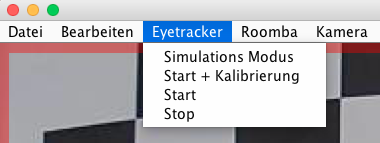
\includegraphics[width=1\textwidth]
      {bilder/implementierung/eyetracker.png} 
      %\subcaption{Objekterkennunsmodus}
      \label{fig:l3} 
   \end{minipage}%
   \hfill
   \begin{minipage}[t]{.4\linewidth} 
      \centering 
      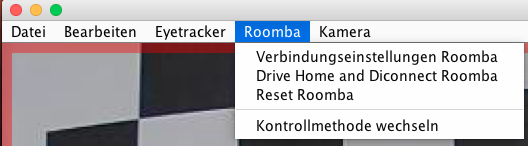
\includegraphics[width=1\textwidth]
      {bilder/implementierung/roomba.png} 
      %\subcaption{Steuerungsmodus}
      \label{fig:l2} 
   \end{minipage}%
   %\hfill
\begin{minipage}[t]{.4\linewidth} 
      \centering 
      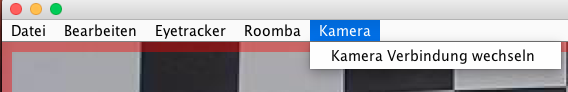
\includegraphics[width=1\textwidth]{bilder/implementierung/kamera.png} 
      %\subcaption{Betrachtungsmodus}
      \label{fig:l1} 
   \end{minipage}% 
   \hfill

\end{center}
\caption{Menüleiste mit den möglichen Menüauswahlpunkten.}
\label{fig:menu}
\end{figure}

Eine weitere, in \acs{abb}~\ref{fig:diskretModeKomp} nicht dargestellte Komponente, ist ein Pop-up-artiges Informationsfenster, das als ein visueller Feedbackmechanismus beispielsweise bei der erfolgreichen Kalibrierung des Eyetrackers oder bei der Verbindung mit dem mobilen Roboter für eine kurze definierte Zeitdauer erscheint. Dieser Mechanismus wurde von der Vorgängerversion übernommen, wobei in der aktuellen Version auf das akustische Feedback verzichtet wurde, siehe \acs{abb}~\ref{fig:info}, \vgl~\cite{Eidam2015}.

\begin{figure}[ht]
\begin{center}
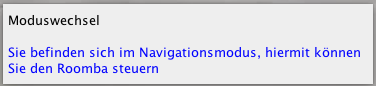
\includegraphics[width=0.6\textwidth]{bilder/implementierung/Infoframe.png}
\end{center}
\caption{Beispiel des Informationsframe als visueller Feedbackmechanismus. Mit \enquote{Navigantionsmodus} wird im vorliegenden Fall der \textsc{Steuerungsmodus} bezeichnet.}
\label{fig:info}
\end{figure}
\subsection{Gestaltung der Kontrollmodi}
\label{subsection:gestKontroll}
Die Benutzeroberfläche stellt drei unterschiedliche Modi zur Verfügung, durch die der Benutzer mit einer definierten Augengeste navigieren kann. Vorgesehen wurden die Modi:
\begin{enumerate}
\item \textsc{Betrachtungsmodus}
\item \textsc{Steuerungsmodus}
\item \textsc{Objekterkennungsmodus}
\end{enumerate}
Jeder dieser drei Modi stellt einen unterschiedlichen Funktionsumfang bereit, wobei der \textsc{Objekterkennungsmodus} nur demonstrativ für die geplante Objekterkennungsfunktion einer zukünftigen Softwarevariante steht, jedoch im aktuellen Prototyp keinerlei Funktionen bereithält. Die Modi werden durch eine unterschiedliche farbliche Außenranddarstellung gekennzeichnet (siehe~\acs{abb}~\ref{fig:modi}). Zunächst wird ein \textsc{Betrachtungsmodus} angeboten, der der Orientierung im Blickbereich dient und für die Interaktion mit der Menüleiste fungieren kann. Hierbei ist keine Steuerung des Telepräsenzrobotersytems möglich. Durch eine vertikale Blickbewegung erfolgt der Wechsel in den \textsc{Steuerungsmodus}. Hier findet die eigentliche Steuerung des \acs{tps} statt, wobei innerhalb des \textsc{Steuerungsmodus} mittels des Menüpunktes \enquote{Kontrollmethode wechseln} aus dem Menüleistenpunkt \enquote{Eyetracker} alternierend zwischen den beiden Steuermethoden (diskret und kontinuierlich) gewechselt werden kann, siehe~\acs{abb}~\ref{fig:menu}. 
Erfolgt eine weitere vertikale Blickgeste, so findet ein Wechsel in den \textsc{Objekterkennungsmodus} des Systems statt. Eine erneute vertikale Blickgeste führt zurück in den \textsc{Betrachtungsmodus}.
\begin{figure}[ht]
\begin{center}
\begin{minipage}[b]{.3\linewidth} 
      \centering 
      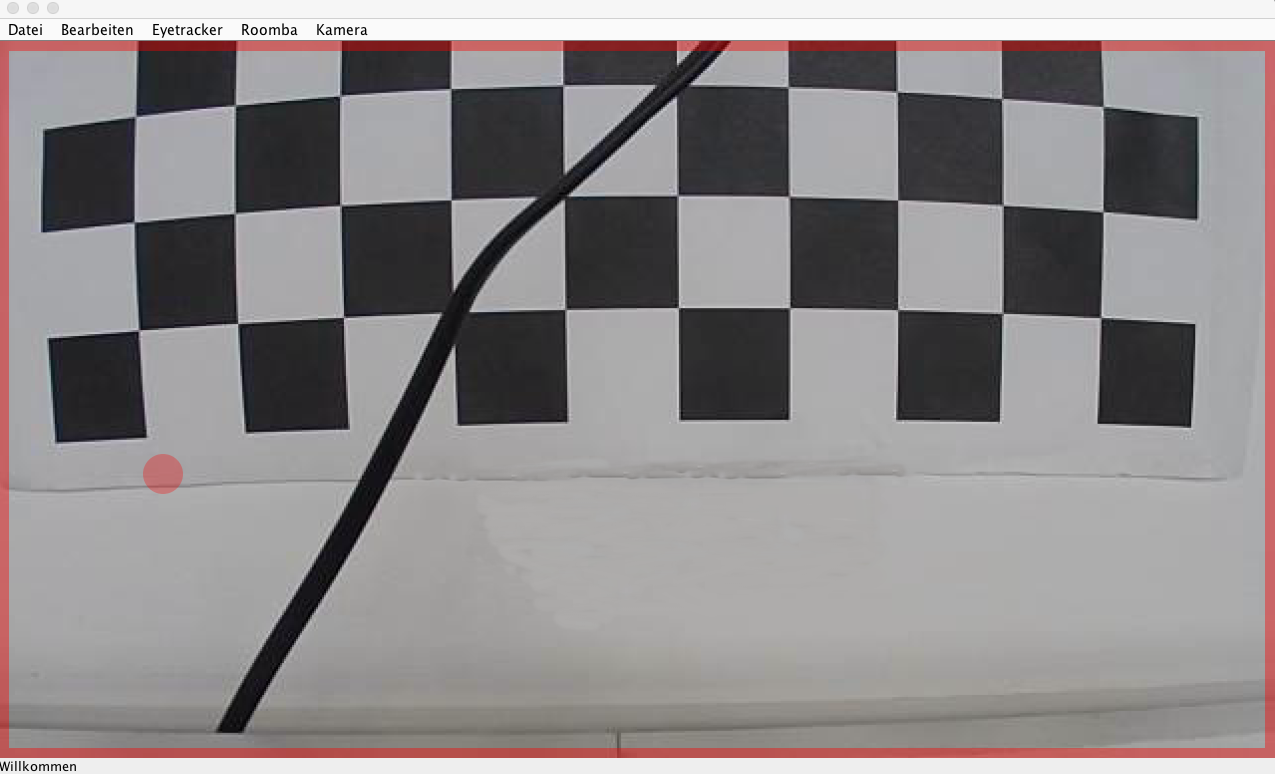
\includegraphics[width=1\textwidth]{bilder/implementierung/rot.png} 
      \subcaption{Betrachtungsmodus}
      \label{fig:l1} 
   \end{minipage}% 
   \hfill
   \begin{minipage}[b]{.3\linewidth} 
      \centering 
      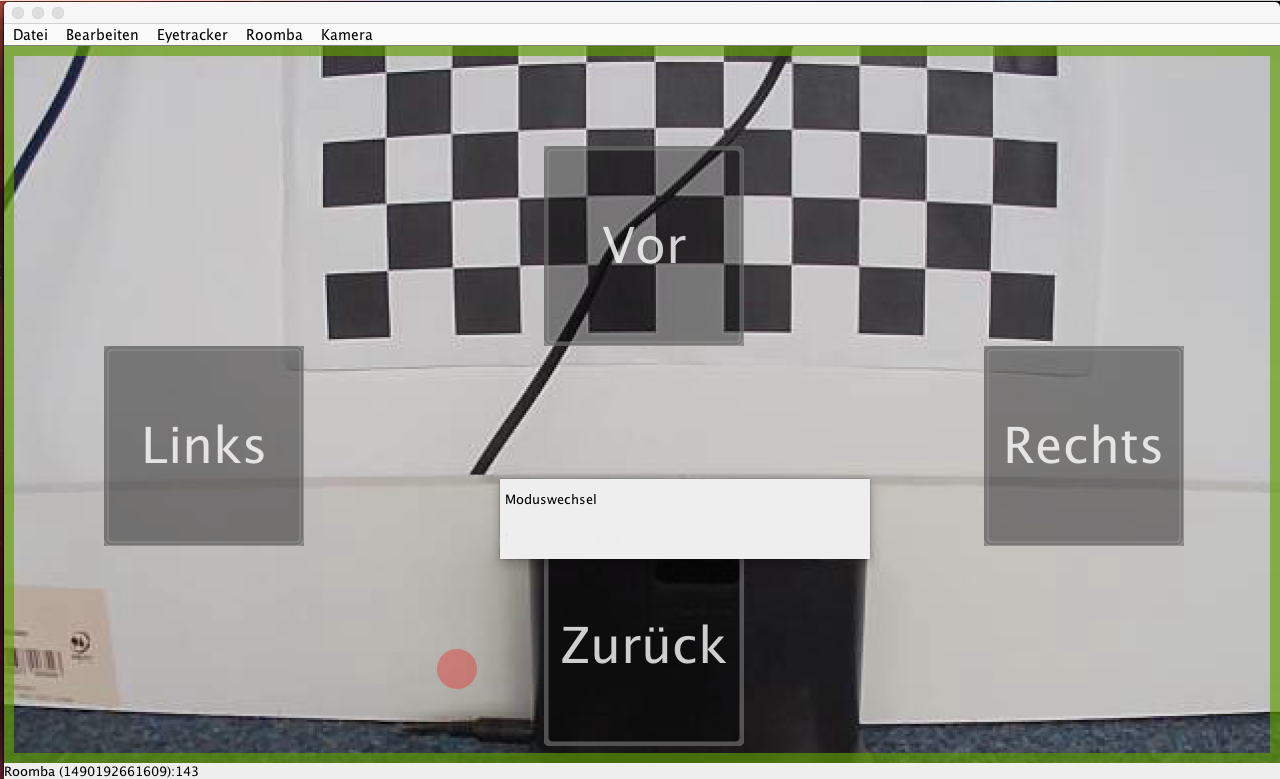
\includegraphics[width=1\textwidth]
      {bilder/implementierung/gruen.png} 
      \subcaption{Steuerungsmodus}
      \label{fig:l2} 
   \end{minipage}%
   \hfill
   \begin{minipage}[b]{.3\linewidth} 
      \centering 
      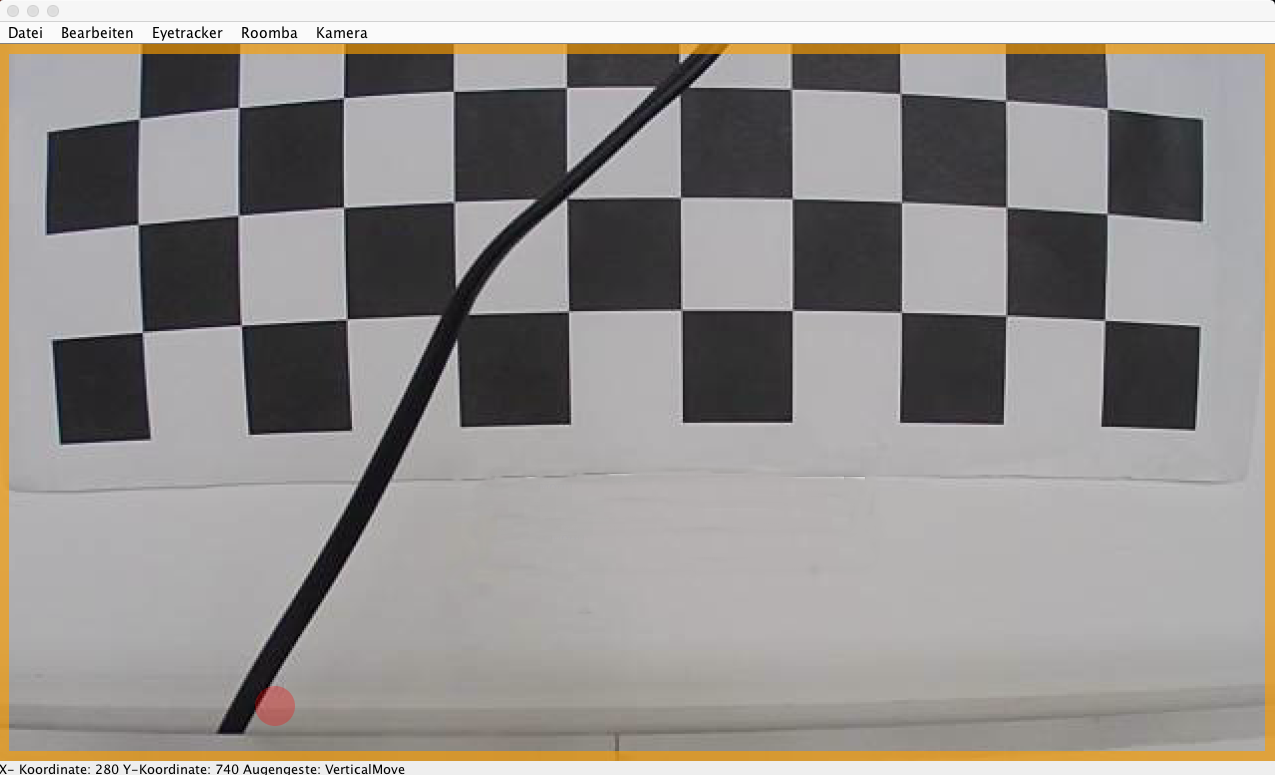
\includegraphics[width=1\textwidth]
      {bilder/implementierung/gelb.png} 
      \subcaption{Objekterkennungsmodus}
      \label{fig:l3} 
   \end{minipage}%
   \hfill
\end{center}
\caption{Darstellung der drei unterschiedlichen Kontrollmodi. Betrachtungsmodus~(rot), Steuerungsmodus~(grün), Objekterkennungsmodus (gelb).}
\label{fig:modi}
\end{figure}
Bei jedem Wechsel des Modus wird ein Informationsfenster als visueller Feedbackmechanismus angeboten. Dieser dient dazu, den aktuellen Modus zu benennen und dadurch eine einfachere Orientierung in der Programmführung zu ermöglichen.

\subsection{Gestaltung der diskreten Steuerung}
\label{subsection:gestDisk}
Zur Umsetzung der diskreten Steuerung wurden vier Steuerelemente (vor, zurück, links, rechts) auf dem Bildschirm angeordnet, siehe \acs{abb}~\ref{fig:diskretMode}. Diese wurden hierbei als teiltransparente Elemente konzipiert, um den Bereich \enquote{hinter} den Elementen nicht zu verdecken und möglichst den gesamten Blickbereich des \acs{tps} zur Orientierung und zur Bewegungsplanung zu nutzen. Der aktuelle \acs{por} des Benutzers wurde mittels eines teiltransparenten roten Punktes dargestellt und bewegt sich in Abhängigkeit der Blickbewegung, \vgl~\acs{abb}~\ref{fig:diskretMode}. Bei der Größenauswahl der Elemente wurde auf eine ausreichende Relation zwischen den elementfreien Bereichen der Blickfläche und der Größe der Elemente geachtet. Im Prototyp nehmen die Steuerelemente ca. 20 \% der Blickfläche ein und ermöglichen so einen größtenteils unbeeinträchtigten Blick auf die Bildfläche der Telepräsenskamera, gleichzeit sind die Flächen groß genug, um mittels der Augenbewegung selektiert zu werden. 
\begin{figure}[ht]
\begin{center}
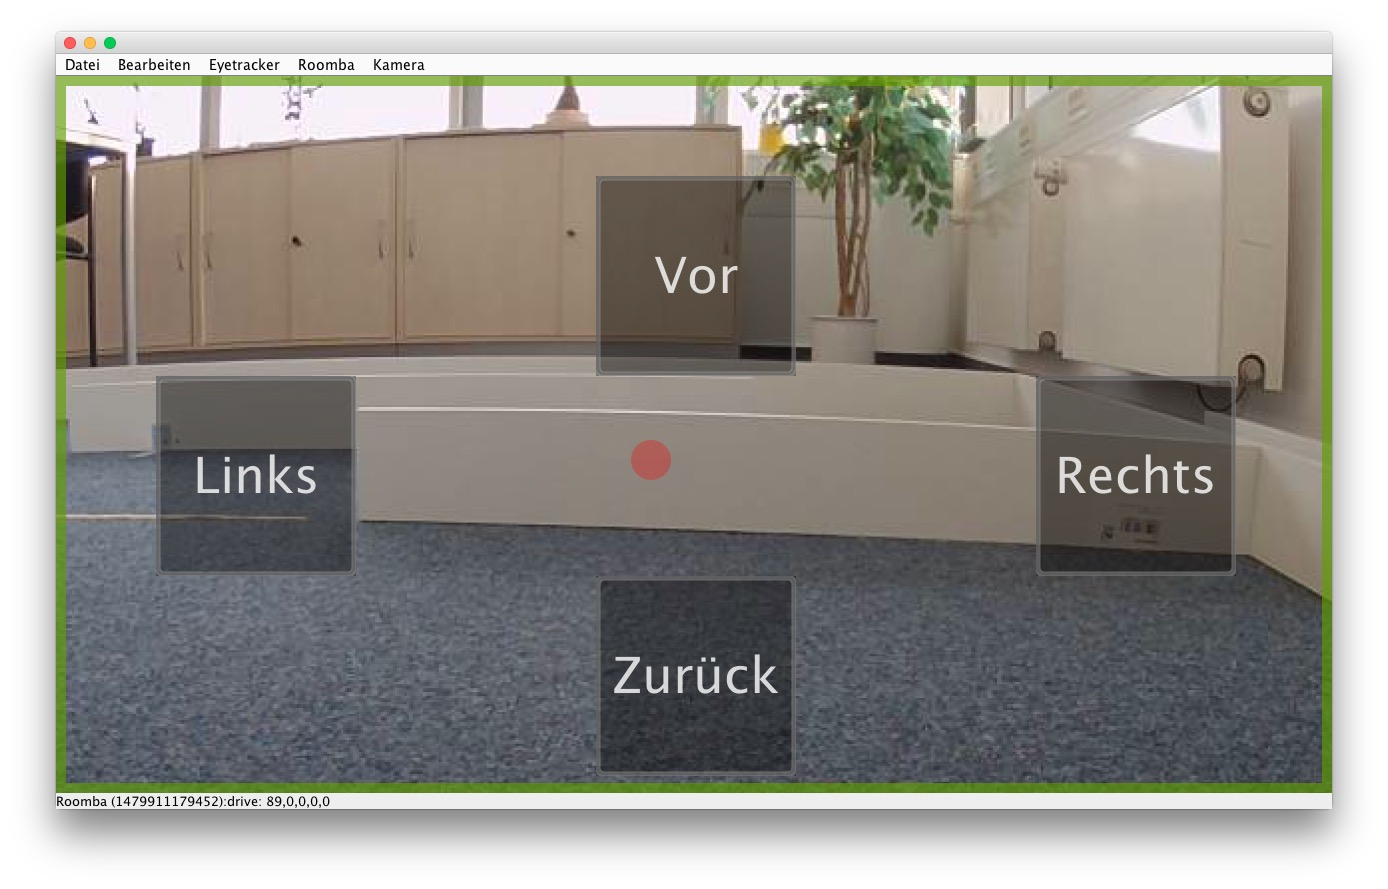
\includegraphics[width=\textwidth, height=100mm]{bilder/implementierung/diskretMode.JPG}
\end{center}
\caption{Darstellung der diskreten Steuerelemente (vor, zurück, links, rechts).}
\label{fig:diskretMode}
\end{figure}

\subsection{Gestaltung der kontinuierlichen Steuerung}
Zur Gestaltung der kontinuierlichen Steuerung wurde ein \enquote{Koordinatenkreuz} im Zentrum des Blickbereiches positioniert, siehe \acs{abb}~\ref{fig:contMode}. Ein farblich hervorgehobener Bereich in der Mitte des Blickfeldes wurde als \enquote{Neutralzone} konzipiert. Dadurch sollten das Midas-Touch-Problem reduziert und nur bewusste Steuerabsichten des Benutzers umgesetzt werden. Wurde der \acs{por} des Benutzers in diesen Bereich gerichtet, blieb das \acs{tps} unbewegt an seiner aktuellen Position stehen. Die Positionierung eines \enquote{Koordinatenkreuzes} sollte die Position der Neutralstellung veranschaulichen. Die Steuersignale wurden im Hinblick auf die Geschwindigkeits- und Richtungsamplitude anhand einer farblichen Abszissen- und Ordinatenachse in Abhängigkeit der Steuerbewegung abgebildet (in \acs{abb}~\ref{fig:contMode} durch den gelb und grünlich dargestellten Abschnitt im Bereich der \enquote{Neutralzone} nur schwer zu erkennen). Durch das Koordinatenkreuz ist es ferner möglich, eine Einteilung in vier verschiedenen Quadranten des Blickfeldes vorzunehmen (genauere Ausführungen im Abschnitt \ref{subsection:kontSt}).
\begin{figure}[ht]
\begin{center}
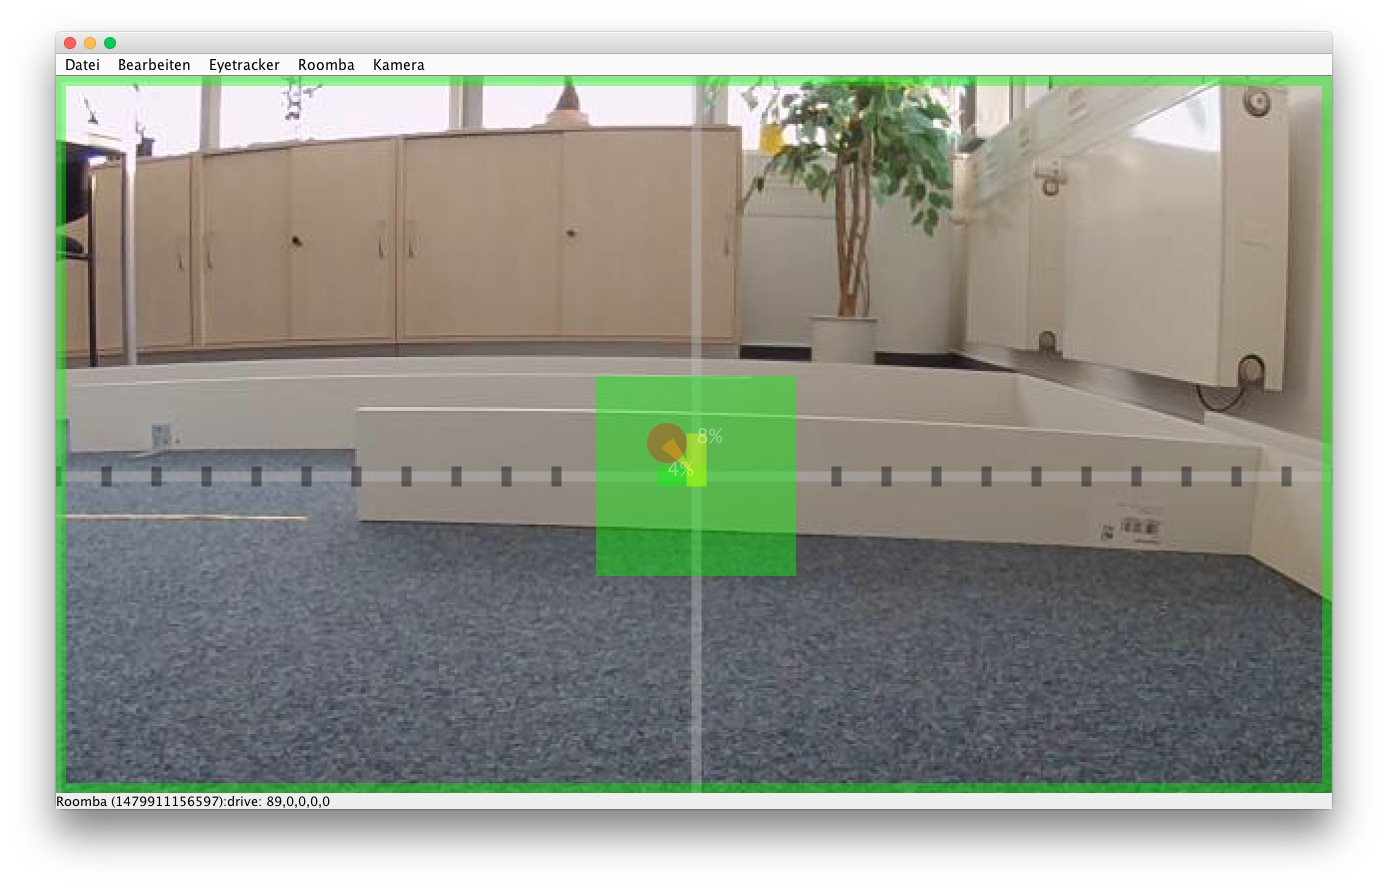
\includegraphics[width=\textwidth]{bilder/implementierung/continuousMode.JPG}
\end{center}
\caption{Darstellung der kontinuierlichen Steuerelemente. Zentral ist die \enquote{Neutralzone} farblich markiert. Dieser Bereich erzeugt keine Steuerbefehle und dient der Reduktion des Midas-Touch- Problems. Der rot markierte Punkt im Zentrum zeigt den \acs{por} des Benutzers.}
\label{fig:contMode}
\end{figure}


\section{Telepräsenzrobotersystem (TPS)}
\label{section:tpsI}
\subsection{iRobot Roomba 620}
Für die vorliegende Arbeit wurde als \tp ein \enquote{handelsüblicher} autonomer Staubsaugerroboter (Roomba 620) der Firma iRobot® Corporation benutzt, siehe \acs{abb}~\ref{fig:roomba}. Der Roomba ist seitens des Herstellers so konzipiert worden, dass dieser ohne technische Vorkenntnisse des Benutzers relativ einfach verwendet werden kann und hierbei weitgehend autonom funktioniert. Er eignet sich aufgrund einer seit 2005 vom Hersteller bereitgestellten offenen Schnittstellendokumentation (iRoomba Create Open Interface (OI))~\cite{IRobot2010} hervorragend zur Augmentation als \tp. Der Roomba ist somit durch die angebotene Befehlsstruktur der OI im Verhalten vielfältig zu kontrollieren. Um die für ein \tp benötigte visuelle Komponente zu gewährleisten, wurde der Roboter um eine zentrisch angeordnete Kamera erweitert, siehe \acs{abb}~\ref{fig:subroomba} auf Seite \pageref{fig:subroomba}. Zur Netzwerkkommunikation und entfernten Steuerung wurde ein Access-Point an der seriellen Schnittstelle des mobilen Roboters angebracht (\vgl~\acs{abb}~\ref{fig:subroomba}). Die vorinstallierten Bürsten des Staubsaugerroboters wurden aufgrund der Geräuschentwicklung und der fehlenden Funktion während des Gebrauchs entfernt. 

\begin{figure}[ht]
\begin{minipage}[b]{\linewidth} 
      \centering 
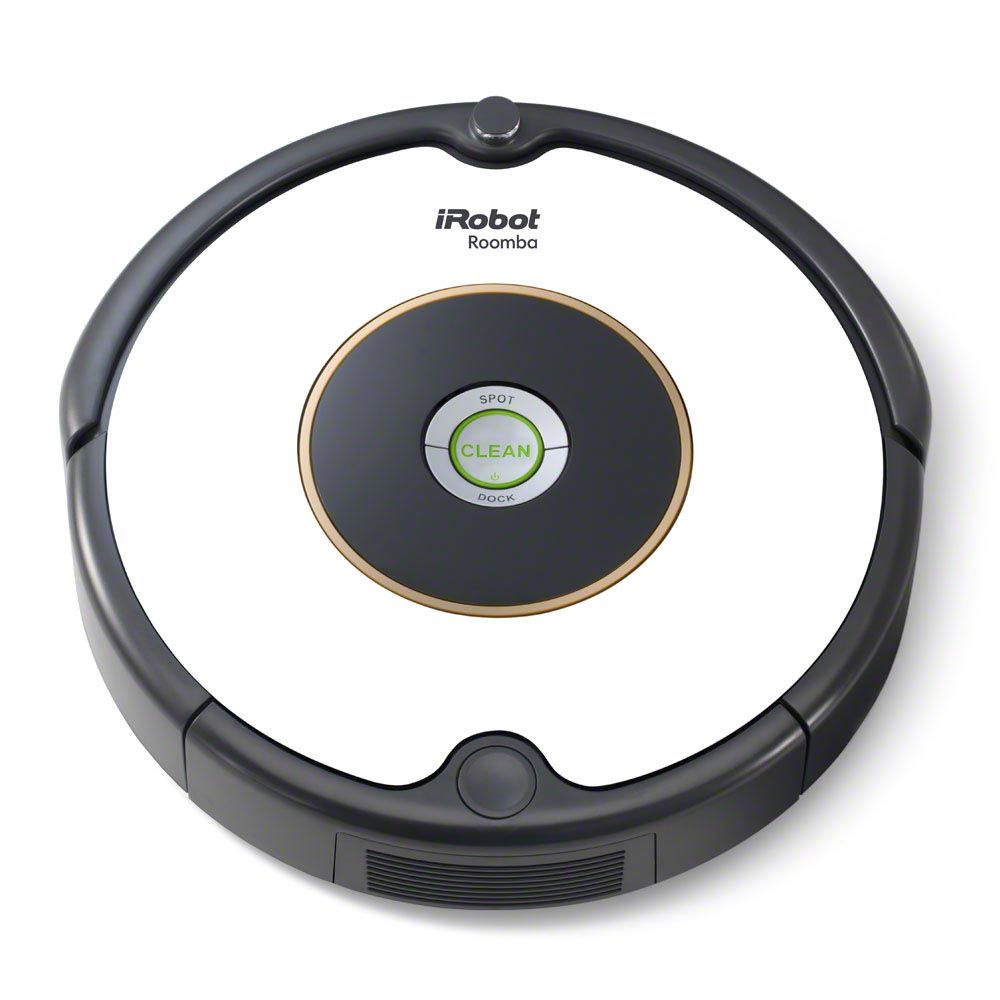
\includegraphics[scale=0.15]{bilder/implementierung/Roomba.jpg}\label{fig:roombaSub1} 
   \end{minipage}% 
   \hfill
\caption{Roomba 620 als Staubsaugerroboter. (Bild: Webshop des Herstellers, \url{http://shop.irobot.de/roomba-staubsstaubsaugerroboter-roomba-605/R605040.html?cgid=de\&lang=de_DE} (letzter Aufruf: 23. November 2016))}
\label{fig:roomba}
\end{figure}

Nachfolgend erfolgt die Vorstellung der Schnittstellendokumentation mit der Einführung in die bereitgestellten Kontrollmodi und der, für die Implementierung benötigten Befehle.


\subsection{Modi des iRoomba Create Open Interface (OI)}
Während der Benutzung des Roombas befindet sich dieser in einem der vier unterschiedlichen Kontrollmodi: Off, Passiv, Safe und Full \cite{IRobot2010}. Die Modi legen fest, welche Verhaltensweisen seitens des Roombas vorgesehen sind und wie auf eintreffende Befehle, (siehe Abschnitt~\ref{subsction:befehlsstruktur}) reagiert wird. Folgend werden die vier Modi des Roombas, wie in den Angaben des Herstellers beschrieben,
dargestellt \cite{IRobot2010}:
\begin{description}
\item[\enquote{Off}-Modus] Darin befindet sich der Roomba nach einem Batteriewechsel oder nach dem ersten Anschalten. Der Roomba erwartet in diesem Modus einen \enquote{Start}-Befehl (siehe Abschnitt~\ref{subsction:befehlsstruktur}) und wechselt nach Erhalten des Befehls in den \enquote{Passiv}-Modus.

\item[\enquote{Passiv}-Modus] Nach Erhalt eines \enquote{Start}-Befehls (siehe Abschnitt~\ref{subsction:befehlsstruktur}) wechselt der Roomba in diesen Modus. Hierbei können Sensordaten ausgelesen werden, jedoch sind keine Steuerbefehle für die vorhandenen Steuerkomponenten (Lautsprecher, Motoren, Leuchtdioden) möglich. 

\item[\enquote{Safe}-Modus] Der Safe-Modus bietet die gleiche Funktionalität wie der Passiv-Modus. Zusätzlich kann der Roomba dabei nun kontrolliert und gezielt gesteuert werden. Alle vorhandenen Befehle sind nun unter der Voraussetzung ausführbar, dass keines der folgenden sicherheitsrelevanten Ereignisse eingetreten ist: 
\begin{itemize}
\item Ein Abhang wird während der Vorwärts- oder Rückwärtsbewegung erkannt.
\item Ein Rad steckt fest.
\item Das Ladegerät ist angeschlossen und der Roomba wird geladen.
\end{itemize}
Tritt eines dieser sicherheitsrelevanten Ereignisse auf, werden alle Motoren umgehend gestoppt und der Roomba wird in den \enquote{Passiv}-Modus versetzt.

\item[\enquote{Full}-Modus] Durch das Senden eines \enquote{Full}-Befehls (siehe Abschnitt~\ref{subsction:befehlsstruktur}) erhält der Benutzer in vollem Umfang Zugang zu den Steuerkomponenten (Lautsprecher, Motoren, Leuchtdioden). Die sicherheitsrelevanten Ereignisse werden hierbei nicht überwacht.
\end{description}

\acl{abb}~\ref{fig:roombamodi} verdeutlicht die \og Kontrollmodi und ihre Zustandsänderungen in Abhängigkeit bestimmter Ereignisse.

\begin{figure}[ht]
  \centering
  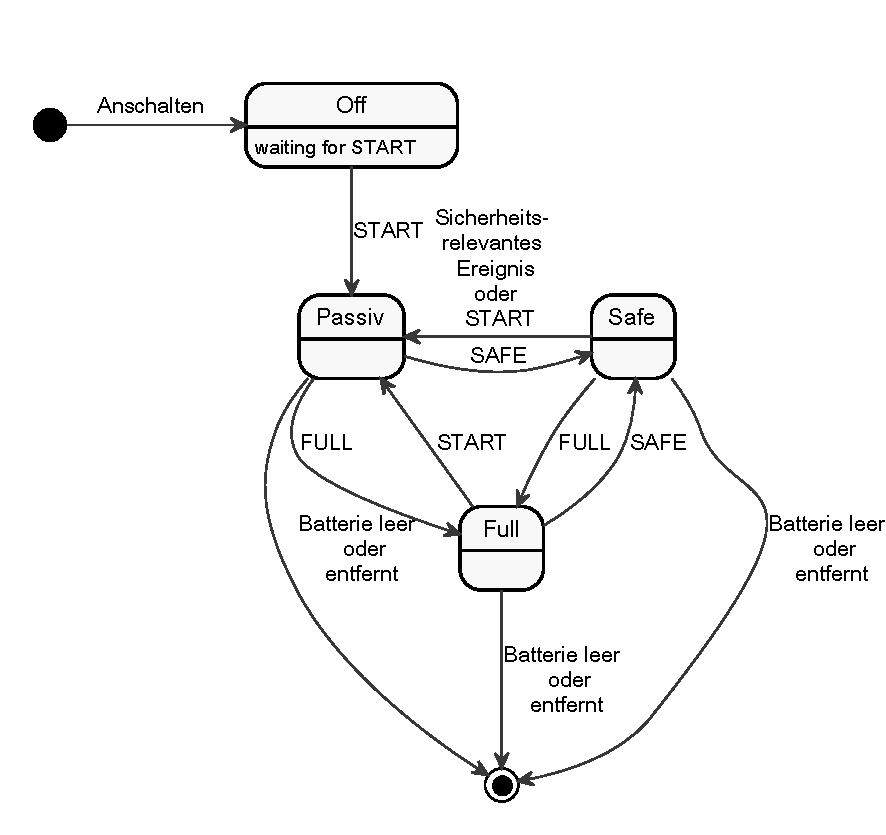
\includegraphics[width=0.6\textwidth]{bilder/implementierung/neuablauf2.pdf}
\caption{Darstellung der vier unterschiedlichen Kontrollmodi des Roombas und der Zustandsübergänge.}
\label{fig:roombamodi}
\end{figure}

\subsection{Befehlsstruktur des iRoomba Create Open Interface (OI)}
\label{subsction:befehlsstruktur}
Der Befehlsumfang, der durch das OI angeboten wird, bietet eine umfangreiche Interaktionsmöglichkeit mit den Sensoren und Steuerkomponenten des Roombas. Für die Implementierung des Softwareprototyps wurde nur eine kleine Anzahl der bereitgestellten Befehle verwendet. So wurde die Netzwerkkommunikation nur unilateral in Richtung des \acs{tps} genutzt. Auf das Auslesen der Senordaten des Roombas wurde aufgrund begrenzter Kapazitäten in Bezug auf die parallele bilaterale Kommunikation des angebrachten Access-Points verzichtet. Die nachfolgende Auflistung führt dadurch nur die für die Implementierung verwendeten Befehle auf. Für eine vollständige Auflistung sei auf die ausführlichen Angaben des Herstellers verwiesen (\vgl \cite{IRobot2010}). 
\begin{description}
\item \textbf{Modusbefehle}
\begin{itemize}
\item[\textsc{Start}] (Opcode: 128) (Datenbytes: 0)
\item[\textsc{Safe}] (Opcode: 131) (Datenbytes: 0)
\item[\textsc{Full}] (Opcode: 132) (Datenbytes: 0)
\item[\textsc{Dock}] (Opcode: 143) (Datenbytes: 0)
\end{itemize}
\item \textbf{Fahrbefehle}
\begin{itemize}
\item [\textsc{Drive}] (Opcode: 137) (Datenbytes: 4)
\item [\textsc{Drive} \textsc{Direct}] (Opcode: 145) (Datenbytes: 4)
\end{itemize}
\end{description}
Jeder OI-Befehl beginnt mit einem Ein-Byte großen Befehlsopcode, der den gewünschten Befehl codiert. In Abhängigkeit des Befehlsopcodes werden zusätzlich ein oder mehrere weitere Datenbytes als Argument des Befehls benötigt.
\begin{equation*}
\noindent \color{black} \underbrace{\textbf{|OPCODE|}}_{\substack{\text{Befehlsauswahl}}}\hfill \color{black}\underbrace{\textbf{|Datenbyte 1|}\hfill \textbf{|Datenbyte 2|} \hfill \textbf{|Datenbyte 3|}\hfill \textbf{|Datenbyte 4|}}_{\substack{\text{Variable Anzahl der Datenbytes in Abhänigkeit des Befehlsopcods}}} \hfill 
\end{equation*}

Viele Befehle, wie beispielsweise der oben bereits genannte \textsc{Start}-Befehl~(Opcode:~128), benötigen keine zusätzlichen Datenbytes. Dies trifft auch auf die Gruppe der Modus-Befehle, wie beispielsweise auf den \textsc{Safe}-Befehl~(Opcode:~131), der den Roomba in den \enquote{Safe}-Modus versetzt, oder auf den \textsc{Full}-Befehl~(Opcode:~132), womit der Roomba in den \enquote{Full}-Modus wechselt, zu.

Für die Umsetzung der diskreten und kontinuierlichen Steuerung wurden zwei unterschiedliche Steuerungsbefehle verwendet. Für die diskrete Steuerung bot sich die Funk\-tions\-weise des \textsc{Drive}-Befehls~(Opcode:~137) an und bei der kontinuierlichen Steuerung wurde die Funktion des \textsc{Drive Direct}-Befehls~(Opcode:~145) verwendet, deren allgemeine Beschreibung hier nun folgen. Die konkrete Anwendung folgt in den Abschnitten~\ref{subsection:diskSt} \bzw \ref{subsection:kontSt}.

\subsubsection{\textsc{DRIVE}-Befehl (Opcode:~137)}
Für die Steuerung mittels \textsc{Drive}-Befehls (Opcode:~137) wurde die Ansteuerung der beiden Radmotoren des Roombas durch die Angabe zweier Argumente realisiert (Geschwindigkeit, Radius), \vgl Listing~\ref{lst:drive}.
Hierbei erfolgte die Steuerung durch die Angabe einer durch zwei Bytes codierten \textit{Geschwindigkeit}, im Bereich von -500 mm/s bis \mathplus 500 mm/s, kombiniert mit der Angabe eines, durch weitere zwei Bytes codierten \textit{Radius} im Bereich von -2000 mm bis \mathplus 2000 mm. Daraus ergibt sich für den \textsc{Drive}-Befehl die allgemeine \textit{sequenzielle Struktur} des Befehls:
\begin{equation*}
\begin{split}
\underbrace{\underbrace{\text{|137|}}_{\substack{\text{\text{1 Byte}}}}}_{\substack{\text{\textsc{opcode}}}} \underbrace{\underbrace{\text{|höherwertiges Byte|}}_{\substack{\text{1 Byte}}} \underbrace{\text{|niederwertiges Byte|}}_{\substack{\text{1 Byte}}}}_{\substack{\text{\textsc{Geschwindigkeit}}}} \underbrace{\underbrace{\text{|höherwertiges Byte|}}_{\substack{\text{1 Byte}}} \underbrace{\text{|niederwertiges Byte|}}_{\substack{\text{1 Byte}}}}_{\substack{\text{\textsc{Radius}}}}
\end{split}
\end{equation*}

Anhand der allgemeinen Struktur des \textsc{Drive}-Befehls kann man erkennen, dass zusätzlich zum Opcode-Byte vier weitere Datenbytes notwendig sind, die als zwei vorzeichenbehaftete 16-Bit-Zahlen in Zweierkomplementdarstellung vorliegen. Dabei erkennt man ferner, dass eine Big-Endian-Byte-Reihenfolge vorgesehen ist und dass das höchstwertige Byte zuerst angegeben werden muss. Ist es beispielsweise vorgesehen, den Roomba mit einer Geschwindigkeit von 200 mm/s in Rückwärtsrichtung (Geschwindigkeit mit negativem Vorzeichen) zu bewegen und gleichzeitig in einem Radius von 500 mm zu drehen, ergibt sich folgende Bytesequenz des Befehls \cite{IRobot2010}:
\begin{beispiel}{Beispielsequenz eines \textsc{Drive}-Befehls: [137] [255] [56] [1] [244]} \\
\centering
\(
\underbrace{\color{orange}\underbrace{\underbrace{\text{\textsc{ Opcode }}}_{\substack{\text{\textsc{Drive}}}}}_{\substack{\text{\textsc{|137|}}}}
\color{blue}\underbrace{\underbrace{\underbrace{\text{\textsc{ Geschwindigkeit }}}_{\color{blue}\substack{\text{-200 mm/s}}}}_{\color{blue}\substack{hex FF38}}}_{\color{blue}\substack{\underbrace{hex FF}_{\substack{|255|}}\underbrace{hex 38}_{\substack{|56|}}}}\color{black}\underbrace{\underbrace{\underbrace{\text{\textsc{ Radius }}}_{\substack{\text{500 mm}}}}_{\substack{hex 01F4}}}_{\substack{\underbrace{hex 01}_{\substack{|1|}}\underbrace{hex F4}_{\substack{|244|}}}}} \)\\
\( [137] [255] [56] [1] [244] \)
\label{exa:drive}
\end{beispiel}

Der \textsc{Drive}-Befehl stellt für einige Bewegungsrichtungen,- wie die Drehung nach links oder rechts,- und die Geradausfahrt in Vorwärts- und Rückwärtsrichtung,- spezielle Werte des Radius-Parameters bereit (\vgl~\cite{IRobot2010}):

\begin{itemize}
  \item Gerade = 32768 oder 32767 = hex 8000 oder 7FFF (\vgl~Listing~\ref{lst:vorruck})
  \item Drehung nach rechts = hex FFFF (\vgl~Listing~\ref{lst:rotrechts})
  \item Drehung nach links = hex 0001 (\vgl~Listing~\ref{lst:rotlinks})
\end{itemize}

Der \textsc{Drive}-Befehl kann, wie oben erwähnt, nur während der Ausführung im \enquote{Safe}- oder \enquote{Full}-Modus verwendet werden. Das \og Beispiel zeigt die allgemeine Befehlsstruktur des von der OI bereitgestellten \textsc{Drive}-Befehls~(Opcode:~137). 

\subsubsection{\textsc{DRIVE} \textsc{DIRECT}-Befehl (Opcode:~145)}
Der \textsc{Drive}~\textsc{Direct}-Befehl (Opcode:~145) unterscheidet sich zum \og \textsc{Drive}-Befehl dahingehend, dass die Ansteuerung der einzelnen Radsteuermotoren für jedes Rad einzeln möglich ist, \vgl auch Listing~\ref{lst:drivedirect}. Dadurch lässt sich die für die kontinuierliche Steuerung notwendige differenzierte kontinuierliche geschwindigkeits- und richtungsabhängige Befehlscodierung in einem einfachen Algorithmus implementieren, siehe Abschnitt~\ref{subsection:kontSt}. Es folgt die allgemeine \textit{sequenzielle Struktur} des \textsc{Drive}~\textsc{Direct}-Befehls~(Opcode:~145):
\begin{equation*}
\begin{split}
\underbrace{\underbrace{\text{|145|}}_{\substack{\text{\text{1 Byte}}}}}_{\substack{\text{\textsc{opcode}}}} \underbrace{\underbrace{\text{|höherwertiges Byte|}}_{\substack{\text{1 Byte}}} \underbrace{\text{|niederwertiges Byte|}}_{\substack{\text{1 Byte}}}}_{\substack{\text{\textsc{Geschwindigkeit rechtes Rad}}}} \underbrace{\underbrace{\text{|höherwertiges Byte|}}_{\substack{\text{1 Byte}}} \underbrace{\text{|niederwertiges Byte|}}_{\substack{\text{1 Byte}}}}_{\substack{\text{\textsc{Geschwindigkeit linkes Rad}}}}
\end{split}
\end{equation*}

Anhand seiner allgemeinen Struktur des \textsc{Drive} \textsc{Direct}-Befehls erkennt man, dass genau wie beim \textsc{Drive}-Befehl zusätzlich zum Opcode-Byte vier weitere Datenbytes benötigt werden. Hierbei handelt es sich auch um zwei 16-Bit Zahlen in Zweierkomplementärdarstellung und in Big-Endian-Byte-Reihenfolge.
Ein konkretes Beispiel verdeutlicht die Nutzung des \textsc{Drive} \textsc{Direct}-Befehls:

\begin{beispiel}{Beispielsequenz eines \textsc{Drive} \textsc{Direct}-Befehls: [145] [0] [200] [0] [200]} \\
%\textbf{[137] [255] [56] [1] [244]} \\ 
\centering
\(\color{orange}\underbrace{\text{|145|}}_{\substack{\text{\textsc{Drive}\textsc{Direct }}}}\color{blue}\underbrace{\underbrace{\underbrace{\text{|0|}}_{\substack{\text{hex 00}}} \underbrace{\text{|200|}}_{\substack{\text{hex C8}}}}_{\substack{= \text{200 mm/s}}}}_{\substack{\text{\textsc{Geschwindigkeit rechtes Rad }}}} \color{black}\underbrace{\underbrace{\underbrace{\text{|0|}}_{\substack{\text{hex 00}}} \underbrace{\text{|200|}}_{\substack{\text{hex C8}}}}_{\substack{= \text{200 mm/s}}}}_{\substack{\text{\textsc{Geschwindigkeit linkes Rad }}}}\)
\label{exa:driveDirect}
\end{beispiel}

Die erzeugte Bewegung der Befehlssequenz im Beispiel~\ref{exa:driveDirect} entspräche einer Fahrt mit einer Geschwindigkeit von 200 mm/s geradeaus, da beide Motoren dieselbe Geschwindigkeit umsetzen.

Die Umsetzung des \textsc{Drive} \textsc{Direct}-Befehls kann ebenfalls nur während der Ausführung im \enquote{Safe}- oder \enquote{Full}-Modus erfolgen. 

Nachfolgend wird auf die konkrete Umsetzung der beschriebenen Befehle (\textsc{Drive}-Befehl~(Opcode:~137), \textsc{Drive} \textsc{Direct}-Befehl (Opcode:~145)) für die Steuermodelle eingegangen und die Anwendung der Befehle nochmals verdeutlicht.

\section{Umsetzung der Robotersteuerung des Prototyps}
\label{subsection:robotsteuerung}
Nachdem die Befehlsstruktur der Schnittstelle des Roombas im vorherigen Abschnitt beschrieben wurde, folgt nun die konkrete Anwendung der Befehle im Rahmen der beiden Steuerungsmethoden. 

\subsection{Umsetzung der diskreten Steuermethode}
\label{subsection:diskSt}
Wie bereits in Abschnitt \ref{subsection:gestDisk} beschrieben, wurden zur Umsetzung der diskreten Steuermethode vier Steuerelemente (vor, zurück, links, rechts) konzipiert.
Wird der Blick \bzw der \acs{por} des Benutzers in einem Bereich eines der Steuerelemente gelenkt, so wird der entsprechende Befehl an den mobilen Roboter gesendet. Hierbei wird beispielsweise durch das \enquote{vor}- Steuerelement das Signal einer translationalen Bewegung in Vorwärtsrichtung in der aktuellen Geschwindigkeit an den mobilen Roboter gesendet. Durch das Steuerelement \enquote{zurück} entsprechend in Rückwärtsrichtung. Verlässt der \acs{por} des Benutzers den Bereich des Steuerelements, wird dementsprechend kein weiteres Signal gesendet und das \acs{tps} verbleibt an der aktuellen Position. Wird durch eine Blickgeste das \enquote{links}- oder \enquote{rechts}-Steuerelement ausgewählt, so wird ein Befehl zur Rotation nach links oder nach rechts an den mobilen Roboter gesendet. Eine translationale Bewegung findet hierbei nicht statt, der mobile Roboter dreht sich an der aktuellen Position. Dabei wird beim Verlassen der Blickbewegung des jeweiligen Steuerelements auch die entsprechende Rotationsbewegungsbewegung gestoppt. Durch diese Art der Steuerung werden durch alternierende Rotation und Translationsbewegungen jegliche Positionen auf dem Feld erreicht und die Voraussetzungen für eine Umsetzung der Parcoursbewältigungsaufgabe sind prinzipiell gegeben. Wie bereits im Abschnitt~\ref{subsction:befehlsstruktur} dargelegt, wurde zur Realisierung der Steuerkomponenten der diskreten Steuerung der Befehl \textsc{Drive} verwendet. Hierbei wurde jede Steuerkomponente (vor, zurück, links, rechts) für die beabsichtigte Bewegungsrichtung durch die feste Zuteilung der Befehlsparameter (Geschwindigkeit, Radius) für eine der vier möglichen Bewegungen zugewiesen. Die Geschwindigkeit des mobilen Roboters ließ sich in den allgemeinen Systemeinstellungen für die diskrete Steuerung festlegen. Zur Erzeugung der Bewegungsrichtungen in einer Geschwindigkeit von 200 mm/s wurden folgende Befehlssequenzen erzeugt: 
\begin{description}
\item [Vorwärts:] [137] [0] [200] [128] [0]
\item [Rückwärts:] [137] [255] [56] [128] [0]
\item [Drehung nach rechts:] [137] [0] [200] [255] [255]
\item [Drehung nach links:] [137] [0] [200] [0] [1]
\end{description}

Die Realisierung des \enquote{Panikschalters} für die diskrete Steuerungsmethode wurde dadurch ermöglicht, dass eine Steuerung des mobilen Roboters nur durch das jeweilige Betätigen einer Steuerkomponente erfolgte. Es war ausreichend, den \acs{por} in einen der Bereiche ohne Steuerelemente zu lenken, um im Notfall keine Steuersignale zu senden. Ferner ist es möglich, durch einen Lidschluss die Steuerung zu pausieren und sich im Blickbereich \enquote{umzusehen}, bevor man die Steuerung mittels eines erneuten Lidschlusses erneut startet. 

\begin{comment}
Programmiertechnisch wurde dies mittels folgender Implementierungen umgesetzt. Die Methoden sind von der ..., des Projekts Hacking Roomba abgeleitet \cite{Kurt2007}.
\lstinputlisting[language=java, numbers=left, firstline=336, lastline=342,frame=single,breaklines=true, style=myCustomJavaStyle, caption={Vorwärts- und Rückwertsbewegung}, label=lst:vorruck]{code/ARoomba.java}

Wie in Listing \ref{lst:vorruck} dargestellt wird die Vorwärts  \bzw Rückwärtsbewegung durch das Vorzeichen der Geschwindigkeit definiert. Die Angabe des Parameters \(0x8000 = [128] [0]\) des Radius definiert wie bereits in Abschnitt \ref{subsction:befehlsstruktur} beschrieben die Fahrt geradeaus. Die dargestellten Fallunterscheidungen dienen der Limitation auf die maximal positive und negative Geschwindigkeit von 500 mm/s.

\lstinputlisting[language=java, numbers=left, firstline=321, lastline=323,frame=single,breaklines=true, style=myCustomJavaStyle, caption={Rotationsbewegung in Uhrzeigersinn}, label=lst:rotrechts]{code/ARoomba.java}

\lstinputlisting[language=java, numbers=left, firstline=311, lastline=313,frame=single,breaklines=true, style=myCustomJavaStyle, caption={Rotationsbewegung entgegen des Uhrzeigersinn},label=lst:rotlinks]{code/ARoomba.java}

Wie in Listing \ref{lst:rotrechts} und \ref{lst:rotlinks} dargestellt werden die Rotationsbewegungen durch Angabe des Parameters \(\text{0xffff = [255] [255]}\) und \(\text{0x0001 = [0] [1]}\) des Radius definiert wie auch bereits in Abschnitt \ref{subsction:befehlsstruktur} beschrieben wurde. Somit wird bei der Betätigung der Steuerelemente \enquote{Rechts} und \enquote{Links} der in Listing \ref{lst:rotrechts} und \ref{lst:rotlinks} Code aufgerufen.

\lstinputlisting[language=java, numbers=left, firstline=390, lastline=394,frame=single,breaklines=true, style=myCustomJavaStyle, caption={Drive-Befehl},label=lst:drive]{code/ARoomba.java}

Listing \ref{lst:drive} zeigt die Umsetzung des \textsc{Drive}-Befehls in Java. Die Umsetzung eines Stoppbefehls ist in Listing \ref{lst:stop} gezeigt. Hierbei wird eine Befehl mit der Geschwindigkeit Null und dem Radius Null erzeugt.

\lstinputlisting[language=java, numbers=left, firstline=177, lastline=179,frame=single,breaklines=true, style=myCustomJavaStyle, caption={Stop-Befehl},label=lst:stop]{code/ARoomba.java}
\end{comment}

\subsection{Umsetzung der kontinuierlichen Steuermethode}
\label{subsection:kontSt}
Im Vergleich zur diskreten Steuerung wurden, wie bereits \og, mittels der kontinuierlichen Steuerung keine fest zugewiesenen Befehle erzeugt. Vielmehr sollte es für den Benutzer möglich sein, durch entsprechende Augenpositionierung die Geschwindigkeit und die Richtung während der Fahrt flexibel zu variieren. Möglich ist dies durch den beschriebenen \textsc{Drive} \textsc{Direct}-Befehl. Hierbei wird der \acs{por} des Benutzers durch eine Umrechnung in die Geschwindigkeit beider Radmotoren übersetzt. Eine Richtungsänderung der Bewegung kann, wie \og, durch unterschiedliche Geschwindigkeiten der beiden Radmotoren erzielt werden.

Zur Verdeutlichung der Geschwindigkeitsberechnung der Radmotoren während unterschiedlicher Positionen des \acs{por} sei auf die grafischen Beispiele in \acs{abb}~\ref{fig:allkontModus} verwiesen.

\begin{figure}[ht]
   \begin{minipage}[b]{.5\linewidth} 
      \centering 
      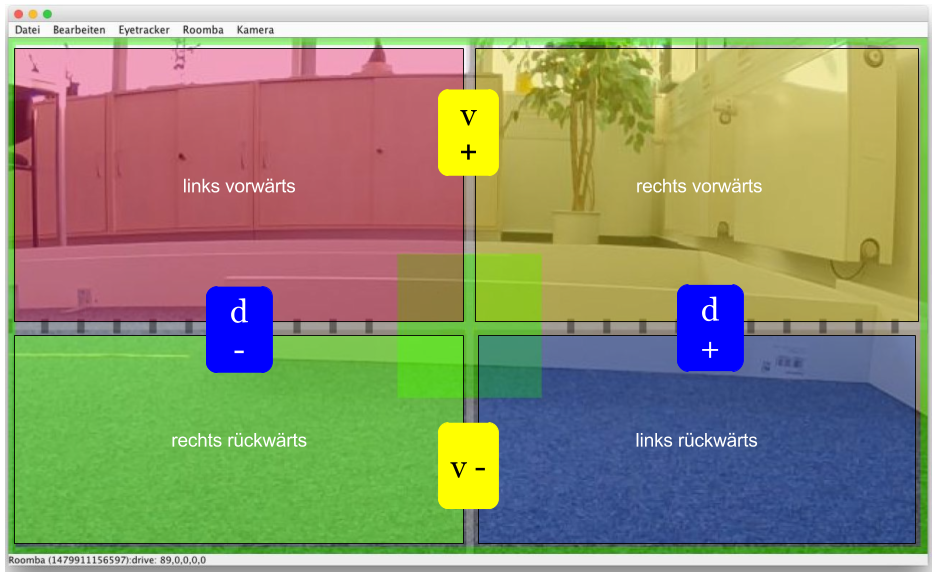
\includegraphics[width=1\textwidth]{bilder/implementierung/richtungen.png} 
      \subcaption{Neutrale Zone}\label{fig:1} 
   \end{minipage}% 
   \hfill
   \begin{minipage}[b]{.5\linewidth} 
      \centering 
      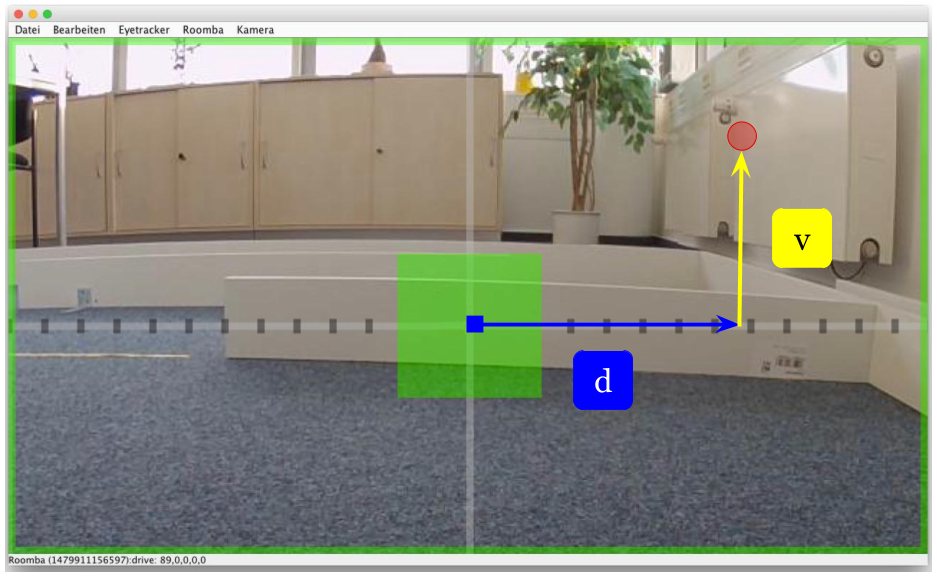
\includegraphics[width=1\textwidth]{bilder/implementierung/rechtsDrive.png} 
      \subcaption{Rechts Vorne}\label{fig:2} 
   \end{minipage}%
   \hfill
   \begin{minipage}[b]{.5\linewidth} 
      \centering 
      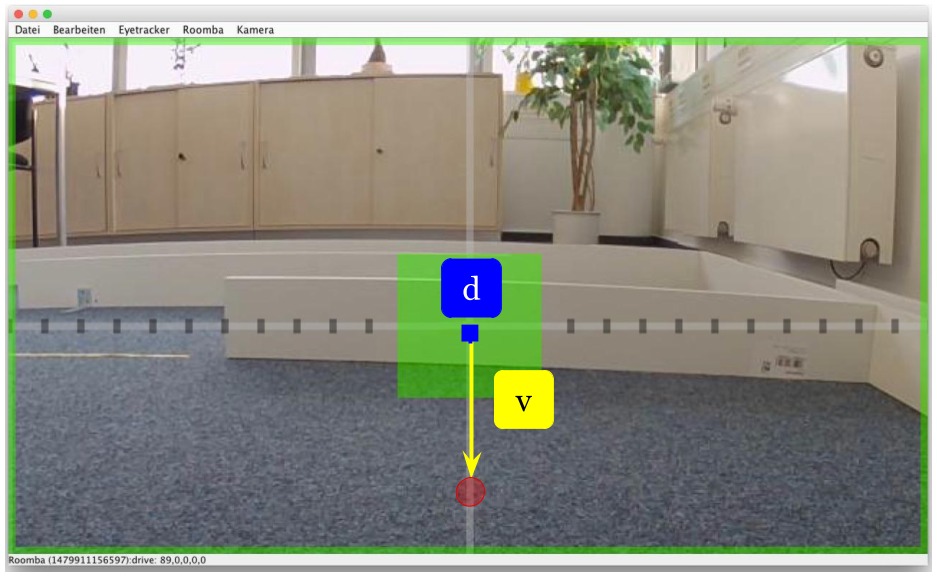
\includegraphics[width=1\textwidth]{bilder/implementierung/ruckDrive.png} 
      \subcaption{Rückwärts}\label{fig:3} 
   \end{minipage}%
   \hfill
   \begin{minipage}[b]{.5\linewidth} 
    \centering 
	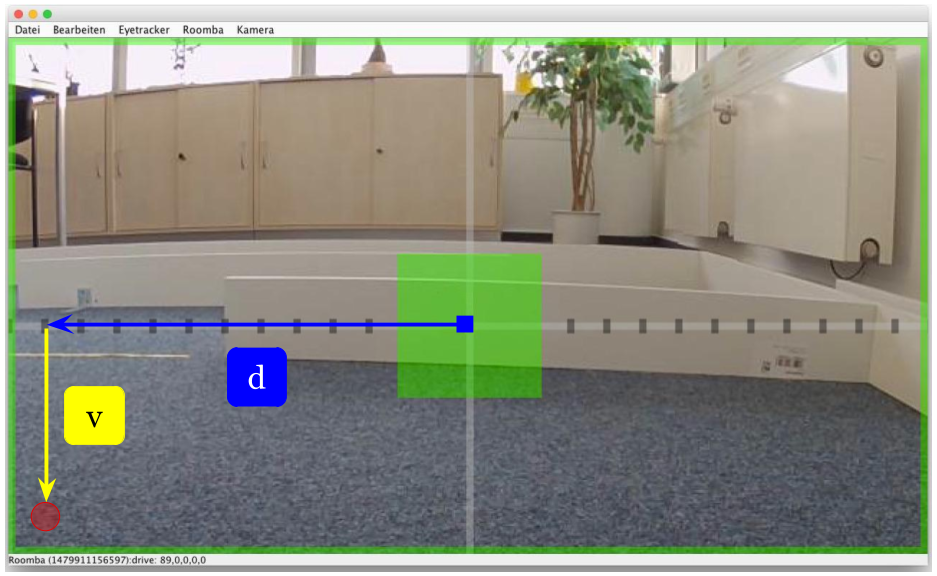
\includegraphics[width=1\textwidth]{bilder/implementierung/linksDrive.png} 
      \subcaption{Links hinten}\label{fig:4} 
   \end{minipage}%
   \hfill
   \caption{Ausgewählte Steuersignale der kontinuierlichen Steuermethode. Blickbewegung in y-Richtung (in Relation zum Mittelpunkt des Koordinatenkreuzes) als $v$ bezeichnet. Blickbewegung in x-Richtung (in Relation zum Mittelpunkt des Koordinatenkreuzes) als $d$ bezeichnet. \textbf{\subref{fig:1}}~zeigt die Wertentwicklung der beiden Variablen in Abhängigkeit der Blickbewegung.}\label{fig:allkontModus} 
\end{figure} 

Der \enquote{Ausschlag} der Blickbewegung in y-Richtung (in Relation zum Mittelpunkt des Koordinatenkreuzes), in \acs{abb}~\ref{fig:allkontModus} als $v$ bezeichnet, definiert die Geschwindigkeit der Radmotoren. Die Blickbewegung innerhalb der oberen Hälfte des Blickfeldes, getrennt durch die Abszisse des Koordinatenkreuzes, erzeugt eine Vorwärtsbewegung der Räder des \acs{tps}. Die Blickbewegung innerhalb der unteren Hälfte des Blickfeldes dementsprechend eine Rückwärtsbewegung. In Abhängigkeit des Abstandes in x-Richtung (in Relation zum Mittelpunkt des Koordinatenkreuzes), in \acs{abb}~\ref{fig:allkontModus} als $d$ bezeichnet, werden nach den folgenden Formeln die einzelnen Radgeschwindigkeiten (rechtes Rad~$V_{r}$, linkes Rad~$V_{l}$) berechnet und somit Richtungsänderungen ermöglicht:
\begin{equation}
\begin{split}
V_{r} = v - d \\\
V_{l} = v + d
\end{split}
\label{eq:formel}
\end{equation}

Wird der Blick beispielsweise in den rechten oberen Bereich des Blickfeldes gerichtet (gelber Bereich, \vgl \acs{abb}~\ref{fig:allkontModus}), resultiert nach Gleichung \ref{eq:formel} eine Reduktion des positiven Geschwindigkeitsfaktors~$v$ des rechten Rades~$V_{r}$ um den positiven Faktor~$d$. Gleichzeitig addiert sich zum Geschwindigkeitsfaktor~$v$ des linken Rades~$V_{l}$ der positive Faktor~$d$ hinzu. Die resultierende Bewegung ist demnach eine nach vorn und rechts gerichtete Bewegung des \acs{tps}.

Für den oben links gelegenen Bereich (roter Bereich, \vgl~\acs{abb}~\ref{fig:allkontModus}) ergibt sich aufgrund der Gleichung und des negativen Faktors~$d$ entsprechend die Bewegung des \acs{tps} nach links vorn.  Blickbewegungen, beispielsweise in den unteren linken Blickbereich (grüner Bereich, \vgl~\acs{abb}~\ref{fig:allkontModus}), führen nach Formel~\ref{eq:formel} aufgrund des jetzt negativen Faktors~$v$ und des negativen Faktor~$d$ zu einer schnelleren Rückwertsdrehung des linken Rades~$V_{l}$ im Vergleich zum rechten Rades~$V_{r}$ und dadurch zu einer nach rechts gerichteten Rückwärtsbewegung. Hierdurch wird ersichtlich, dass durch die vorkommenden Vorzeichen der Gleichung~\ref{eq:formel} und die Vorzeichen der Faktoren~$v$~und~$d$ ein Wechsel der Drehrichtung während eines vertikalen Blickwechsels selben Seite des Blickfeldes resultiert. Anders als vielleicht intuitiv angenommen, muss, um eine Bewegung des \acs{tps} quasi rückgängig zu machen, eine diagonale Blickbewegung ausgeführt werden und nicht - wie vielleicht vermutet - eine vertikale. Dies wäre lediglich für den Fall einer Umkehr einer Vorwärts- \bzw Rückwärtsbewegung sinnvoll.


Die Umsetzung des \enquote{Panikschalters} wurde dadurch realisiert, dass der mobile Roboter nur außerhalb der \enquote{Neutralzone} Steuersignale erhält. Ferner war es möglich, im Bereich der Neutralzone durch einen Lidschluss die Steuerung der kontinuierlichen Methode zu pausieren und sich im Blickbereich \enquote{umzusehen}, bevor man die Steuerung mittels eines erneuten Lidschlusses im Bereich der Neutralzone erneut starten konnte. Dadurch sollte eine unbeabsichtigte Steuerung vermieden werden. 


\section{Eyetracking-System}
\label{section:eyetrackingI}
Im Rahmen der Steuerung des \acs{tps} im vorliegenden Softwareprototyp erfolgte die Erkennung der Augengesten durch das bereits in der Vorarbeit von Eidam et al. \vgl~\cite{Eidam2015} vorgestellte Eyetracking-System \iV des Unternehmens \acf{smi}, siehe \acs{abb}~\ref{fig:device}. Die präzise Erkennung der Augengesten ist im Hinblick auf die erfolgreiche Steuerung des \acs{tps} entscheidend. Der folgende Abschnitt orientiert sich vornehmlich an den Beschreibungen von Eidam (2015) \vgl~\cite{Eidam2015} und stellt die benötigten Komponenten genauer dar.

\subsection{\iV System und \acf{red}}
Das vorgestellte \acs{red} \acl{et} ermöglicht eine kontaktlose Detektion der Augenbewegungen einer Testperson, da es sich um ein stationäres \acs{et} handelt \cite[S.165]{SMI2011}. Das \acs{et} benutzt zwei Infrarot-LED\footnote{Abkürzung für \textit{light-emitting diode} oder \textit{lichtemittierende Diode}}-Quellen zur Erzeugung der für die Detektion benötigten Cornealreflexe \cite[S.22]{SMI2011} (\vgl Ausführungen in Abschnitt~\ref{section:eyeMet}).

Zusätzlich zum \acs{et} besteht das von \acs{smi} bereitgestellte \iV System noch aus einer \acf{wo} und einem stimuluspräsentierenden PC (SP) \cite[S.23]{SMI2011}.
Ein großer Vorteil des \iV Systems besteht in der Bereitstellung einer Middleware (\iV), die für andere Computer oder Anwendungen die Möglichkeit eröffnet, durch eine Systemschnittstelle mit dem \iV zu interagieren und Daten untereinander auszutauschen \cite{SMI2011}. Diese Middleware ermöglicht mittels Imageprocessing die in Echtzeit ablaufende Analyse der Pupillendetektion, die Entfernung von Artefakten und die Berechnung der \acs{por} basierend auf dem in Abschnitt \ref{section:eyeMet} beschriebenen \enquote{Dark-Pupil}-Verfahren zur Erkennung der Augengeste.  
Das \iV System umfasst hierbei folgende Komponenten, die in der \acs{abb}~\ref{fig:eyetracker} dargestellt sind:

\begin{itemize}
\item \iV \acf{wo} 
\item \acf{spb}
\item \acf{et}
\end{itemize}

\begin{figure}[ht]
\begin{center}
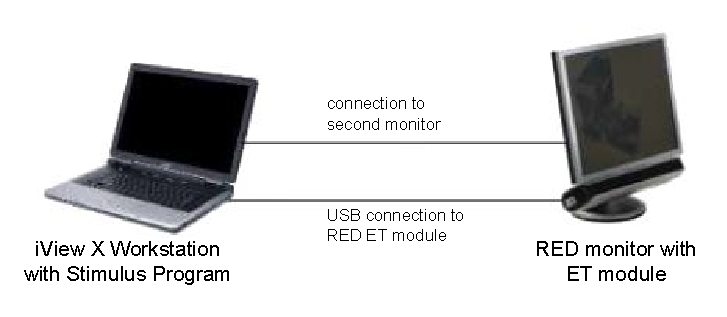
\includegraphics[width=0.7\textwidth]{bilder/implementierung/blick.pdf}
\end{center}
\caption{Die \iV \acf{wo} als Laptop in Verbindung mit dem \acf{spb} und dem \acf{et}. Die \iV Workstation beinhaltet die vorinstallierte Middelware, die zur Kommunikation mit dem Softwareprotyp dient \cite{SMI2011}. (Bild: aus \cite[S.143]{SMI2011})}
\label{fig:eyetracker}
\end{figure}

Nachfolgend wird die Middlewaredokumentation mit der Einführung in die Befehlsstruktur der bereitgestellten Systemschnittstelle vorgestellt.

\subsection{Systemschnittstelle der Middleware (\iV)}
Die Programmierschnittstelle beinhaltet eine Reihe von Befehlen, die es ermöglichen, die Middelware (\iV) durch andere Computer respektive durch den Softwareprototyp zu steuern. Die Kommunikation mit der \iV-Software findet hierbei mittels einer auf \acf{udp} basierenden Netzwerkkommunikation statt \cite[S.439]{SMI2011}. Zur Kommunikation werden nicht alle angebotenen Befehle verwendet. Es erfolgt eine Fokussierung auf die zur Implementierung des Prototyps verwendeten Befehle. Der allgemeine Aufbau eines Befehls besteht aus einer Stringfolge und beginnt bei allen Befehlen mit einer drei Zeichen großen Stringfolge \enquote{ET\_}, gefolgt von einer weiteren, welche die beabsichtigte Aktion spezifiziert \cite[S.484]{SMI2011}\cite{Eidam2015}. In Abhängigkeit der spezifizierten Befehle werden schließlich weitere durch Stringfolgen codierte Parameter angegeben. Die nachfolgende Auflistung führt nur die für die Implementierung verwendeten Befehle aus der Gruppe der Kalibrierungs- und der Datenoutputbefehle auf. Für eine vollständige Auflistung der möglichen Befehle sei auf die ausführlichen Angaben des Herstellers verwiesen (\vgl \cite[484 ff.]{SMI2011}).

\paragraph{Kalibrierungsbefehle}
\begin{itemize}
\item \textbf{ET\_CAL <Punkte> <Binokular Modus>} beginnt die Kalibrierung durch Angabe der zur Kalibrierung notwendigen Punkte durch den Parameter <Punkte>. Mögliche Werte sind (\enquote{2},\enquote{5},\enquote{9},\enquote{13}). Optionaler Parameter nur während der Nutzung des binokularen Modus, wobei \enquote{1} = rechtes Auge, \enquote{2} = linkes Auge repräsentiert \cite[S.489-490]{SMI2011}.
\item \textbf{ET\_CSZ <Breite> <Höhe>} legt die Größe der Kalibrierungsfläche fest, wobei die Fläche durch die Angabe der Pixel mithilfe der Parameter <Breite> und <Höhe> definiert werden \cite[S.493-494]{SMI2011}.
\item \textbf{ET\_PNT <Punktnummer> <X> <Y>} setzt die Koordinaten eines Punktes, charakterisiert durch die <Punktnummer> (Werte zwischen 1 bis 13, siehe Abbildung) und die X- und Y-Koordinate durch die Parameter <X> und <Y> auf dem Bildschirm in Pixel fest \cite[S.503-504]{SMI2011}.
\item \textbf{ET\_CHG <Punktnummer>} signalisiert den Wechsel zum nächsten Kalibierungspunkt durch Angabe der <Punktnummer> \cite[S.490-491]{SMI2011}.
\item \textbf{ET\_ACC} signalisiert das Akzeptieren des aktuellen Kalibierungspunktes und wechselt zum nächsten Kalibrierungspunkt. Dieser Befehl benötigt keinen Parameter \cite[S.487]{SMI2011}.
\item \textbf{ET\_FIN} signalisiert die abgeschlossene Kalibrierung. Dieser Befehl benötigt keine Angabe eines Parameters \cite[S.497]{SMI2011}.
\end{itemize}
\paragraph{Datenoutputbefehle}
\begin{itemize}
\item \textbf{ET\_FRM <Parameterstring : \%TS: \%SX \%SY>} legt das Datenouputformat fest. <Parameterstring> unterscheidet sich in Abhängigkeit des gewählten Modus und setzt sich aus mehreren Teilstrings zusammen (für weitere Angaben siehe \cite[S.500]{SMI2011}):
\begin{itemize}
\item TS: timestamp in Millisekunden ($0 \dots 2^{64}/1000 ms$).
\item SX, SY: X \bzw Y- Wert der Blickposition in Pixel ($\pm 2^{31}$ Pixel).
\end{itemize}
Bei der Deaktivierung des binokularen Modus, wie im Prototyp verwendet, erfolgt trotzdem die Angabe von vier Parametern in der Form: linkes X-linkes Augen.

\item \textbf{ET\_STR} beginnt das kontinuierliche Datenstreaming. Dieser Befehl benötigt keine Angabe eines Parameters
\item \textbf{ET\_EST} beendet das kontinuierliche Datenstreaming. Dieser Befehl benötigt keine Angabe eines Parameters.
\item \textbf{ET\_SPL <Parameterstring : \%TS: \%SX \%SY>} spezifiziert erkannte Datenpunkte durch das im \emph{ET\_FRM}- Befehl festgelegte Format \cite[S.513-514]{SMI2011}).
\end{itemize}


\section{Umsetzung der Augengestenerkennung des Prototyps}
\label{section:augengestenerkennung}
Die Erkennung der Augengesten basiert auf dem von Eidam et al.~(2015, 2016) entwickelten Algorithmen und Prinzipien und wurde im Rahmen dieser Arbeit nahezu unverändert übernommen, \vgl~\cite{Eidam2016,Eidam2015}. Für den aktuellen Prototyp wurde lediglich die Erkennung einer Blickgeste basierend auf dem Algorithmus der Fixationsberechnung hinzugefügt. Damit werden vom vorliegenden Prototypen insgesamt fünf Augengesten erkannt: (1)~\textbf{Fixation}, (2)~\textbf{Blickgeste}, (3)~\textbf{Lidschluss}, (4)~\textbf{vertikale Augengeste}, (5)~\textbf{horizontale Augengeste}. Die \textbf{horizontale Augengeste} wurde wie bei Eidam et al. detektiert, erfüllt im vorliegenden Prototyp jedoch keine Funktion. 

Nachfolgend wird die Umsetzung der Augengesten nach Eidam et al. kurz wiederholend beschrieben \cite{Eidam2016,Eidam2015}.

Prinzipiell werden die vom Eyetracking-System stammenden Koordinaten in einem Koordinatenpuffer mit fester Kapazität geladen und mithilfe der folgenden Algorithmen und Methoden nach jedem Hinzufügen auf das Auftreten einer Augengeste hin untersucht \cite{Eidam2015}. 

\begin{description}
\item[Fixation] Die Registrierung der Fixation wird durch den Bewegungsumfang des \acs{por} berechnet. Bewegt sich der \acs{por} des Benutzers innerhalb eines \textit{definierten Zeitraums} und innerhalb eines \textit{begrenzten Pixelbereichs}, wird eine Fixation erkannt. Die Berechnung des begrenzten Pixelbereichs erfolgt dabei mittels des Algorithmus,~\(|maxX-minX|+|maxY-minY|\), der ein Maß für die Streuung der eingetroffenen Koordinaten ist und auch als Dispersion bezeichnet wird. Hierbei wird der maximale Abstand der detektierten x- und y- Koordinaten addiert und mit einem festgelegten Schwellenwert verglichen. Beim Unterschreiten des Schwellenwerts, also einer Bewegung innerhalb des geforderten Pixelbereichs, wird eine Fixation ausgelöst.
Die Anzahl der zu vergleichenden Koordinaten nach der \og Formel richtet sich nach der gewählten Verweildauer und der Abtastrate des Eyetrackers. Letztere beträgt für den verwendeten Eyetracker 60 Hz. Bei einer Verweildauer von \zB 1000 ms wären dies somit 60 Koordinaten, die durch den \og Algorithmus verglichen werden \cite{Eidam2015}. Durch den Schwellenwert der Dispersion ist es möglich, die Sensitivität\footnote{Grad der Ansprechbarkeit} der Fixation anzupassen \cite[S.295]{SMI2011}. Je näher der Schwellwert dem Wert null liegt, desto exakter musste fixiert werden, um eine Fixationsgeste auszulösen.

\item[Blickgeste] Analog zur Fixationsgeste erfolgt die Umsetzung der Blickgeste auf dem gleichen \og Algorithmus der Dispersionsberechnung. Hierbei unterscheidet sich lediglich die Anzahl der zu vergleichenden Koordinaten. Dies resultiert aus der verkürzten Verweildauer von 100 ms für die Blickgeste. Der Koordinatenpuffer nimmt bei einer Abtastrate von 60 Hz für den Eyetracker 6 Koordinaten und vergleicht diese nach dem \og Prinzip. Damit können pro Sekunde 10 Blickgesten generiert werden.

\item[Lidschluss] Während eines Lidschlusses kommt es aufgrund der kurzzeitigen Verdeckung der Pupille durch das Ober- und Unterlied zu einer temporären Unterbrechung des Koordinatenstroms, wodurch nur Nullwerte vom Eyetracker gesendet werden \cite{Eidam2015}. Dieses passiert auch, wenn der Blick des Benutzers vom Eyetracking-System nicht mehr erkannt wird, beispielsweise weil der Blick vom \acs{et} abgewendet wird. Deshalb muss hier eine Obergrenze definiert werden muss, um nicht jede Blickabwendung zu definieren. Auch zur Unterscheidung eines willkürlichen Lidschlusses als Steuersignal von einem reflexartigen Lidschluss muss eine Ober- \bzw Untergrenze festgelegt werden. Diese Grenzen wurden, wie bei Eidam et al., im Bereich von 250 ms für die untere Grenze und bis 500 ms für die obere Grenze definiert. So werden bei der Abtastrate von 60 Hz mindestens 15 Nullwerte als unterste Grenze benötigt, um eine Lidschlussgeste zu detektieren. Bei einer Anzahl von über 30 Koordinaten ist die Obergrenze erreicht und die Lidschlussgestendetektion wird abgebrochen \cite{Eidam2015}.

\item[Horizontale und vertikale Augengeste]
Für die Detektion der horizontalen und vertikalen Augengesten wird der Koordinatenpuffer hinsichtlich einer Mindestdistanz zwischen zwei entgegensetzt liegenden Punkten in Abhängigkeit der Bildschirmgröße untersucht. Für die horizontale Blickgeste wäre der Abstand der x-Koordinaten beider Punkte entscheidend, für die vertikale Augengeste der Abstand der y-Koordinaten. Gleichzeitig soll die Augenbewegung innerhalb eines Bereiches mit einem Schwellenwert, als \textit{Displacement} bezeichnet, nicht überschritten werden, um diagonale Augenbewegungen nicht mit zu erkennen. Für die horizontale und vertikale Blickgeste beträgt der Mindestabstand 200 Pixel.
\end{description}


\section{Softwarearchitektur}
\label{section:architektur}
\subsection{Überblick}
Im Hinblick darauf wurde die Architektur des Softwareprototyps von Eidam übernommen \cite{Eidam2015,Eidam2016} und um die Steuerung des mobilen Roboterssystems erweitert. Die grundlegende Struktur der Softwareimplementation basiert weiterhin auf einer erweiterten \acf{mvc}-Architektur. Diese wurde um weitere Entwurfsmuster, wie um das Singleton-, Command-, State-, und Beobachtungsmuster erweitert. Ein Überblick der grundlegenden Softwarearchitektur von Eidam (2015) findet sich im Anhang~\ref{chapter:ergabb}.


\subsection{Das Basismodell zur Augengestenerkennung, Modussteuerung und Steuersignalerzeugung}
Auf Grundlage des von Eidam entwickelten Basismodells zur Augen- und Objekterkennung wurde das hier verwendete Modell hinsichtlich der Modussteuerung und der Steuersignalerzeugung angepasst, \vgl~\cite[S.44]{Eidam2015}. Die Erkennung der Augengesten basiert dabei auf den Vorarbeiten von Eidam. Eine Objekterkennung findet im vorliegenden Prototyp nicht statt und unterscheidet sich zum Modell von Eidam. 
Die folgende Beschreibung skizziert grob den Programmablauf während der Laufzeit. Dabei stehen die Augengestenerkennung, Modussteuerung und Steuersignalerzeugung im Fokus. \acl{abb}~\ref{fig:moduskontroll} und \ref{fig:navigationskontrolle} zeigen die wichtigsten beteiligten Klassen. 

\begin{figure}[ht]
\begin{center}
%\missingfigure{Übersichtsaufnahme der Softwarearchitektur}
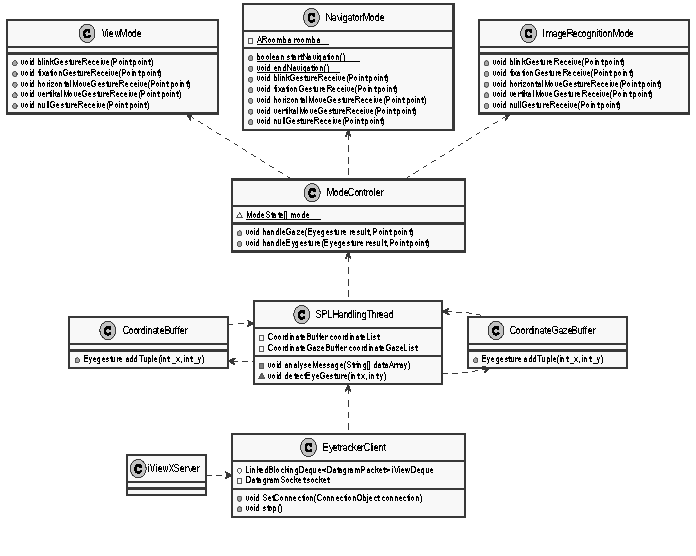
\includegraphics[width=0.9\textwidth]{bilder/uml/moduskontrolle2.pdf}
\end{center}
\caption{Darstellung der wichtigsten Klassen im Zusammenhang mit der Augengestenerkennung und der Modussteuerung.}
\label{fig:moduskontroll}
\end{figure}

\paragraph{Augengestenerkennung}
%\item[]~\hfill
\begin{enumerate}
\item Zunächst erfolgt der Empfang der UDP-Pakete vom \textit{\iV Server} durch den \textit{Eyetracking-Client}. Anschließend analysiert der \textit{SPLHandlingThread} die UDP-Nachricht und extrahiert die Befehle und Koordinaten der Kommunikation. Die Koordinaten werden der Methode \textit{detectEyegesture(int x, int y)} übergeben \cite[S.44]{Eidam2015}. 
\item \textit{detectEyegesture} übergibt die Koordinaten zum einen an die Klasse \textit{CoordinateBuffer}, zur Detektion der Augengeste (Fixation, Lidschluss, horizontal- und vertikale Augengeste) und zum anderen an den \textit{CoordinateGazeBuffer} zur Detektion der Blickgeste. Beide Klassen sind von der Klasse \textit{LinkedList<Point>} abgeleitet und beinhalten die Methode \textit{addTuple(int x, int y)}. Bei erkannter Augengeste erfolgt die Rückmeldung an den \textit{SPLHandlingThread}.
\end{enumerate}

\paragraph{Modussteuerung}
\begin{enumerate}
\setcounter{enumi}{3}
\setcounter{enumii}{1}
\item[\arabic{enumi}.] Die als Singleton angelegte Klasse \textit{ModeController} führt die Funktionalität der erhaltenen Augengeste über die Methode \textit{handleEygesture(Eyegesture result, Point point)} aus. Die Funktionalität der Blickgeste wird über die Methode \textit{handleGaze(Eyegesture result, Point point)} realisiert. \textit{ModeController} ist für die regelrechte Steuerung der unterschiedlichen Modi des Prototypen verantwortlich.
\item[\arabic{enumi}\alph{enumii}.]  Die Methode \textit{handleEygesture} führt je nach erkannter Augengeste (Fixation, Lidschluss, horizontale und vertikale Augengeste), die im Abschnitt \ref{subsection:gestKontroll} beschriebene bereitgestellte Funktionalität der einzelnen Augengesten für jeden der drei Modi aus. Im vorliegenden Prototyp wird ein Moduswechsel durch die horizontale Augengeste angeboten. Die anderen Augengesten bleiben ohne Belegung. Die Modi des Softwareprototyps implementieren alle das \textit{Interface ModeState}, das auf dem State-Entwurfsmuster basiert. 
\setcounter{enumi}{3}
\setcounter{enumii}{2}
\item [\arabic{enumi}\alph{enumii}.] Die Methode \textit{handleGaze} ist für die Steuerung des mobilen Roboters relevant und leitet die detektierten Blickkoordinaten an die Klasse \textit{NavigationsModus} weiter, die die Verbindung zum Roomba herstellt und sie beim Moduswechsel wieder abbaut. 
\end{enumerate}

\paragraph{Steuersignalerzeugung}
\begin{enumerate}
\setcounter{enumi}{3}
\item Die Herstellung einer Verbindung zum \textit{Rommba} erfolgt zunächst durch die Methode \textit{connect(ConnectionRoombaObject roombaConnection)}. Im Anschluss ist es möglich, den Roomba mit Steuerbefehlen zu bewegen, (\vgl~\acs{abb}~\ref{fig:navigationskontrolle}). 
\item In einem nächsten Schritt wird durch die Methode \textit{getCommand()} der Steuerelementeklassen  (\textit{ControlElementDiskret, ControlElementContinuous}) der erzeugte Befehl geliefert, (\vgl~\acs{abb}~\ref{fig:navigationskontrolle}). Dabei produziert jedes Steuerelement nach den in Abschnitt \ref{subsection:diskSt} \bzw \ref{subsection:kontSt} beschrieben Verfahren die Steuerbefehle. Dieses Konzept setzt das Command-Entwurfsmuster um. 
\item Die Klassen \textit{NavigatorMode} führt die Methode \textit{perform()} des aktuellen Befehls (\textit{Command}) aus. Dabei wird die Methode \textit{send(byte[] bytes)} der Klasse \textit{Roomba} realisiert und als Steuerbewegung vom mobilen Roboter umgesetzt (\vgl~\acs{abb}~\ref{fig:navigationskontrolle}). Die Frequenz der Befehlserzeugung ist dabei von der Frequenz der Blickgestendetektion abhängig. 
\end{enumerate}



\begin{figure}[ht]
\begin{center}
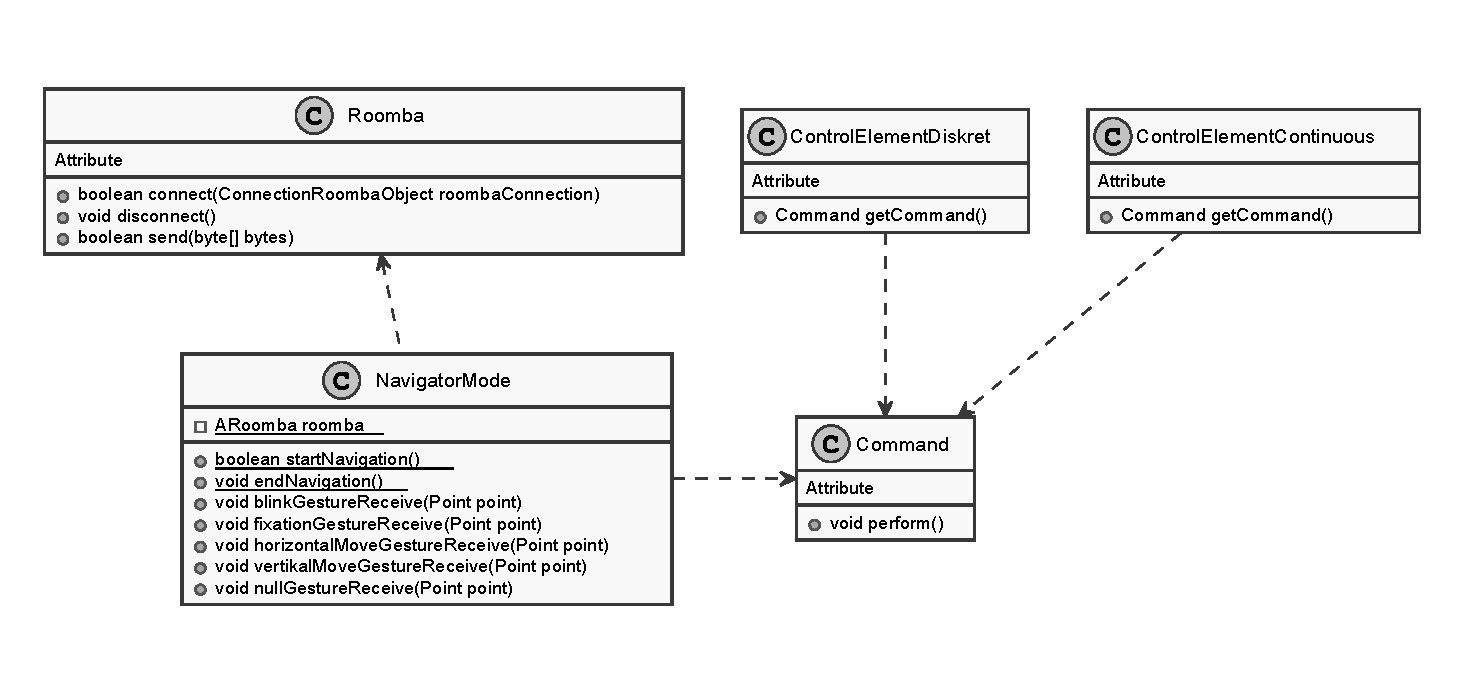
\includegraphics[width=0.9\textwidth]{bilder/uml/navigation.pdf}
\end{center}
\caption{Darstellung der wichtigsten Klassen im Zusammenhang mit der Steuersignalerzeugung.}
\label{fig:navigationskontrolle}
\end{figure}

\section{Technische Umsetzung}
\label{section:techkomp}
Folgender Abschnitt listet die Komponenten, die zur Realisierung des Softwareprototyps verwendet wurden, auf und beschreibt kurz die verwendeten externen Bibliotheken. Die bereits bei Eidam (2015) beschriebene OpenSource Software \textit{MaryTTS} wird im vorliegenden Softwareprototyp aufgrund der übernommenen Softwarearchitektur implementiert, allerdings aufgrund der nicht realisierten Objekterkennung des Prototyp, nicht verwendet \cite{Eidam2015}. 
\subsection{Basis Komponenten}
\begin{description}
\item[Programmierung:] \hfill
\begin{itemize}
\item Programmiersprache Java.
\item \acf{jdk} 1.8.0 Update 91.
\item Swing als Grafikbibliothek.
\item Externe Bibliotheken: \hfill
\begin{description}
\item JavaCV\footnote{Website und Download: \url{https://github.com/bytedeco/javacv} (letzter Aufruf: 15. Juni 2016)} (Version~1.2. [Juni 2016])
\item RoombaComm\footnote{\url{http://hackingroomba.com/code/roombacomm/} (letzter Aufruf: 25. Mai 2016)} \footnote{\url{http://roombahacking.com/software/roombacomm-0.96.zip} (letzter Aufruf: 25. Mai 2016)} (release 0.96 [September 2006]) von Tod E. Kurt und Paul Bouchier.
\end{description}  
\end{itemize}
\item[\acf{ide}:] \hfill
\begin{itemize}
\item Eclipse Java EE IDE for Web Developers (Version: Eclipse Mars.2 Release [4.5.2]).
\item Versionskontrolle durch Eclipse Git (Version: 4.4.1.201607150455-r) .
\end{itemize}
\item[Software-Zielformat]\hfill
\begin{itemize}
\item ausführbare Jar-Datei
\end{itemize}
\end{description}
\subsection{Externe Bibliotheken}
Dieser Abschnitt beschreibt kurz die beiden zusätzlich verwendeten externen Bibliotheken.
\begin{description}
\item[JavaCV (Version~1.2. [Juni 2015])] Zur Umsetzung der Videobilddarstellung des mobilen Roboters, wurde auf die frei zugängliche JavaCV-Bibliothek zurückgegriffen. JavaCV vereint wichtige Bibliotheken aus dem Bereich der Bildverarbeitung und ermöglicht die Codierung und Decodierung eines \acf{mjpeg}-Video-streams. \acs{mjpeg} ist ein Verfahren zur Codierung und Decodierung digitaler Videos, bestehend aus komprimierten Einzelbildern in JPEG-Norm\footnote{Die Bezeichnung \textit{JPEG} resultiert aus dem Namensgebenden Gremium \textit{Joint Photographic Experts Group}, welches 1992 den JPEG Standard (ISO/IEC 10918) entwickelt hat. \url{https://jpeg.org/about.html} (letzter Aufruf: 19. März 2017)}. Die verwendeten Kamera (AXIS M1034-W) stellt diesen Videostream bereit. Entscheidend für die Umsetzung der Videobilddarstellung waren die für die Bildverarbeitung notwendige Programmbibliothek \textit{OpenCV \footnote{\url{http://opencv.org/} (letzter Aufruf: 19. März 2017)}} und das Multimedia Framwork \textit{FFmpeg \footnote{\url{http://ffmpeg.org/} (letzter Aufruf: 19. März 2017)}}. 

Notwendig ist es neben den im JavaCV-Paket enthaltenen jar-Dateien, die Datei \textit{ffmpeg-3.0.2-1.2.jar} zusätzlich mit in das Projekt einzubinden.

\item[RoombaComm (release 0.96 [September 2006])] Zur Realisierung der Kommunikation des Systems mit dem verwendeten Robotersystem Roomba wurde die von Tod Kurt und Paul Bouchier bereitgestellte Java-Bibliothek zur Kommunikation und Kontrolle des Roombas für die Nutzung im Softwareprototyp modifiziert \cite{Kurt2007}.
Verwendung fanden die beiden Klasse:
\begin{itemize}
\item RoombaComm
\item RoombaCommTCPClient
\end{itemize}
\end{description}






\begin{comment}


Für die Steuerung des vorliegenden Prototypen wurde hauptsächlich die, in der Arbeit von Ediam beschriebene, Fixation als Grundlage für die benutzte Blickgeste verwendet \cite{Eidam2015}. Wie bereits im Abschnitt \ref{chapter:grundlagen} beschrieben, ist die Fixation eine Augengeste im Rahmen der Wahrnehmung. Dabei wird die Registrierung der Fixation durch den Bewegungsumfang des \acs{por} berechnet. Bewegt sich der \acs{por} des Benutzers innerhalb eines \textit{definierten Zeitraums} und innerhalb eines begrenzten Blickbereichs, wird eine Fixation erkannt \cite{Eidam2015,SMI2011}. Bei Festlegung sehr kurzer Zeiträume kann die Fixation als Blickgeste interpretiert werden. In der Arbeit von Eidam wurden für den vorliegenden Prototypen zur Steuerung des \acs{tps} die Blickgesten verwendet. Im Hinblick auf eine Nutzung des Systems, für die Möglichkeit einer Interaktion mit Objekten im Bild, ist es sinnvoll die Fixation neben einer reinen Blickgeste als Augengeste zu definieren. 


\subsubsection{Fixation}

\end{comment}